%\documentclass{sig-alternate-05-2015}
\documentclass{llncs}
\usepackage{makeidx}
\usepackage{tabularx,colortbl}
\usepackage[dvipsnames]{xcolor}
\usepackage{flushend}
\usepackage{cite}
\usepackage{amsmath}
%\usepackage{amsthm}
\usepackage{amssymb}
\usepackage{epsfig}
\usepackage{stmaryrd}
\usepackage{url}
\usepackage{multirow}
\usepackage{latexsym}
\usepackage{graphics}
\usepackage{graphicx}
\usepackage{enumitem}
\usepackage{comment}
\usepackage{longtable}
\usepackage{supertabular}
\usepackage{times}
\usepackage{listings}
\usepackage{subfigure}
\usepackage{color}
\usepackage{balance}
\usepackage{xspace}
\usepackage[ruled, vlined, linesnumbered]{algorithm2e}
\usepackage[autostyle]{csquotes}
\usepackage[]{algorithm2e}
%\usepackage[font=large]{caption}



%\theoremstyle{Definition}
%\newtheorem{definition}{Definition}
%%%
%\theoremstyle{Theorem}
%\newtheorem{theorem}{Theorem}


%\newcommand{\definition}{\noindent \textbf{Definition} \citation{}}
%\newcommand{\theorem}{\noindent \textbf{Theorem} \citation{}}
%\newcommand{\lemma}{\noindent \textbf{Lemma} \citation{}}

%\newdef{lemma}{Lemma}
%\newdef{definition}{Definition}
%\newdef{theorem}{Theorem}
%\newdef{corollary}{Corollary}
%\newdef{note}{Note}
%\newdef{axiom}{Axiom}
\newcommand{\mkeyword}[1]{\mbox{\texttt{#1}}}
\DeclareMathOperator{\kuop}{uop}
\DeclareMathOperator{\kbop}{bop}
\DeclareMathOperator{\kite}{ite}
\DeclareMathOperator{\kpre}{pre}
\DeclareMathOperator{\dom}{dom}
\DeclareMathOperator{\ktrue}{true}
\DeclareMathOperator{\kfalse}{false}
\DeclareMathOperator{\kselect}{select}
\DeclareMathOperator{\ran}{range}
\newcommand{\lbb}{[\![}
\newcommand{\rbb}{]\!]}
\newcommand{\expr}{\phi}
\newcommand{\exprS}{\Phi}
\newcommand{\mats}[1]{\textcolor{red}{#1}}
\newcommand{\janet}[1]{\textcolor{blue}{#1}}
\newcommand{\darren}[1]{\textcolor{green}{#1}}
\newcommand{\danielle}[1]{\textcolor{orange}{#1}}

\sloppypar



\begin{document}

\definecolor{gold}{rgb}{0.90,.66,0}
\definecolor{dgreen}{rgb}{0,0.6,0}
\newcommand{\stateequiv}{\equiv_{s}}
\newcommand{\traceequiv}{\equiv_{\sigma}}
\newcommand{\ta}{\text{TA}}
\newcommand{\cta}{\text{TA$_{C}$}}
\newcommand{\tta}{\text{TA$_{T}$}}
\newcommand{\ucalg}{\texttt{\small{IVC\_UC}}}
\newcommand{\ucbfalg}{\texttt{\small{IVC\_UCBF}}}


\title{The Safety Annex for the Architecture Analysis and Design Language}
%
\author{Danielle Stewart\inst{1}
\and Jing (Janet) Liu\inst{2}
\and Michael W. Whalen\inst{1}
\and Darren Cofer\inst{2}
\and Mats Heimdahl\inst{1}
\and Michael Peterson\inst{3}}
\institute{University of Minnesota\\Department of Computer
Science and Engineering\\
\email{dkstewar, whalen, heimdahl}@cs.umn.edu
\and
Collins Aerospace\\
%Advanced Technology Center
Trusted Systems - Engineering and Technology
\\
\email{Jing.Liu, Darren.Cofer}@collins.com
\and
Collins Aerospace\\
%Commercial Systems 
Flight Controls Safety Engineering - Avionics\\
\email{Michael.Peterson}@collins.com
}
\maketitle

\begin{abstract}
%Mats' abstract
Model-based development techniques are increasingly being used in the development of critical systems software. Leveraging the artifacts from model based development in the safety analysis process would be highly desirable to provide accurate analysis and enable cost savings. In particular, architectural and behavioral models provide rich information about the system's operation. In this paper we describe an extension 
to the Architecture Analysis and Design Language (AADL) developed to allow a rich modeling of a system under failure conditions. This \emph{Safety Annex} allows the independent modeling of component failure modes and allows safety engineers to weave various types of faults into the nominal system model. 
The accompanying tool support allows investigation of the propagation of errors from their source to their effect on top level safety properties without the need to add separate propagation specifications; 
it  also supports describing dependent faults that are not captured through the behavioral models, 
e.g., failures correlated due to the physical structure of the system.
We describe the Safety Annex, illustrate its use with a representative example, and discuss and demonstrate the tool support enabling an analyst to investigate the system behavior under failure conditions.	
	

\end{abstract}

\keywords{Model-based systems engineering, fault analysis, safety engineering}

\section{Introduction}

System safety analysis techniques are well established and are a required activity in the development of commercial aircraft and safety-critical ground systems. However, these techniques are based on informal system descriptions that are separate from the actual system design artifacts, and are highly dependent on the skill and intuition of a safety analyst. The lack of precise models of the system architecture and its failure modes often forces safety analysts to devote significant effort to gathering architectural details about the system behavior from multiple sources and embedding this information in safety artifacts, such as fault trees.

While model-based development (MBD) methods are widely used in the aerospace industry, they are generally disconnected from the safety analysis process itself. Formal model-based systems engineering (MBSE) methods and tools~\cite{QFCS15:backes,hilt2013,NFM2012:CoGaMiWhLaLu,DBLP:journals/scp/CimattiT15,Pajic2012,DBLP:conf/adaEurope/SokolskyLC09} now permit system-level requirements to be specified and analyzed early in the development process. These tools can also be used to perform safety analysis based on the system architecture and initial functional decomposition. Design models from which aircraft systems are developed can be integrated into the safety analysis process to help guarantee accurate and consistent results. This integration is especially important as the amount of safety-critical hardware and software in domains such as aerospace, automotive, and medical devices has dramatically increased due to desire for greater autonomy, capability, and connectedness.

Architecture description languages, such as SysML~\cite{SysML} and the Architecture Analysis and Design Language (AADL)~\cite{AADL} are appropriate for capturing system safety information.  There are several tools that currently support reasoning about faults in architecture description languages, such as the AADL error annex~\cite{Larson:2013:IAE:2527269.2527271} and HiP-HOPS for EAST-ADL~\cite{CHEN201391}.  However, these approaches primarily use {\em qualitative} reasoning, in which faults are enumerated and their propagations through system components must be explicitly described.  Given many possible faults, these propagation relationships become complex and it is also difficult to describe temporal properties of faults that evolve over time (e.g., leaky valve or slow divergence of sensor values).

In earlier work, University of Minnesota and Rockwell Collins developed and demonstrated an approach to model-based safety analysis (MBSA) \cite {Joshi05:Dasc,Joshi05:SafeComp,NasaRep:MBSA-Aug05} using the Simulink notation \cite{MathWorks}.  In this approach, a behavioral model of (sometimes simplified) system dynamics was used to reason about the effect of faults.  We believe that this approach allows a natural and implicit notion of fault propagation through the changes in pressure, mode, etc. that describe the system's behavior.  Unlike qualitative approaches, this approach allows uniform reasoning about system functionality and failure behavior, and can describe complex temporal fault behaviors.  On the other hand, Simulink is not an architecture description language, and several system engineering aspects, such as hardware devices and non-functional aspects cannot be easily captured in models.

\iffalse
Over the last five years, several research groups have focused on formal reasoning at the system architecture level, resulting in MBSE tools that incorporate assume-guarantee compositional reasoning techniques~\cite{Trento and Rockwell and UMN}.  These tools allow behavioral reasoning about complex system models, but with substantially greater scalability than previous approaches.
\fi

This paper describes our initial work towards a behavioral approach to MBSA using AADL.  Using assume-guarantee compositional reasoning techniques, we hope to support system safety objectives of ARP4754A and ARP4761.  To make these capabilities accessible to practicing safety engineers, it is necessary to extend modeling notations to better describe failure conditions, interactions, and mitigations, and provide improvements to compositional reasoning approaches focused on the specific needs of system safety analysis.  These extensions involve creating models of fault effects and weaving them into the analysis process.  To a large extent, our work has been an adaptation of the work of Joshi et. al to the AADL modeling language.

To evaluate the effectiveness and practicality of our approach, we developed an architectural model of the Wheel Braking System model in SAE AIR6110.  Starting from a reference AADL model constructed by the SEI instrumented with qualitative safety analysis information~\cite{SEI:AADL}, we added behavioral contracts to the model.  In so doing, we determine that there are errors related to (manually constructed) propagations across components, and also an architecture that contains single points of failure.  We use our analyses to find and fix these errors.

The rest of the paper is organized as follows...





\section{Preliminaries}
\label{sec:prelims}
One of our goals is to transition the tools we have developed into use by the safety engineers who perform safety assessment of avionics products. Therefore, we need to understand how the tools and the models will fit into the existing safety assessment and certification process.
ARP4754A, the Guidelines for Development of Civil Aircraft and Systems~\cite{SAE:ARP4754A}, provides guidance on applying development assurance at each hierarchical level throughout the development life cycle of highly-integrated/complex aircraft systems. It has been recognized by the Federal Aviation Administration (FAA) as an acceptable method to establish the assurance process. The safety assessment process is a starting point at each hierarchical level of the development life cycle and is tightly coupled with the system development and verification processes. It is used to show compliance with certification requirements and for meeting a company's internal safety standards. 

ARP4761, the Guidelines and Methods for Conducting Safety Assessment Process on Civil Airborne Systems and Equipment~\cite{SAE:ARP4761},  identifies a systematic means to show compliance. Among the industry accepted safety assessment processes are Preliminary System Safety Assessment (PSSA) and System Safety Assessment (SSA). PSSA evaluates the system design and defines safety requirements. SSA evaluates the implemented system to show that safety requirements defined in the PSSA are in fact satisfied.

A prerequisite of performing the safety assessment is understanding how the system is intended to work, primarily focusing on the integrity of the outputs and the availability of the system. The safety engineers then use the acquired understanding to conduct safety analysis, construct safety analysis artifacts, and compare the results with established safety objectives and requirements.
Typically equipped with the domain knowledge about the system, but not detailed knowledge of how the software applications are designed, practicing safety engineers find it a time consuming and involved process to acquire the knowledge about the behavior of the software applications hosted in a system and its impact on the overall system behavior.
Industry practitioners have come to realize the benefits of using models in the safety assessment process, and a revision of the ARP4761 to include Model Based Safety Analysis (MBSA) is under way.
Figure~\ref{fig:proposed_safety_process} presents our proposed use of a single unified model to support both system design and safety analysis. It describes both system design and safety-relevant information 
that are kept distinguishable and yet are able to interact with each other. The shared model maintains a living model that captures the current state of the system design as it moves through the development lifecycle, allowing all participants of the ARP4754A process to be able to communicate and review the system design. Safety analysis artifacts can be generated directly from the model, 
providing
the capability to more accurately analyze complex systems.

\begin{figure}[t!]
	\vspace{-0.45in}
	\centering
	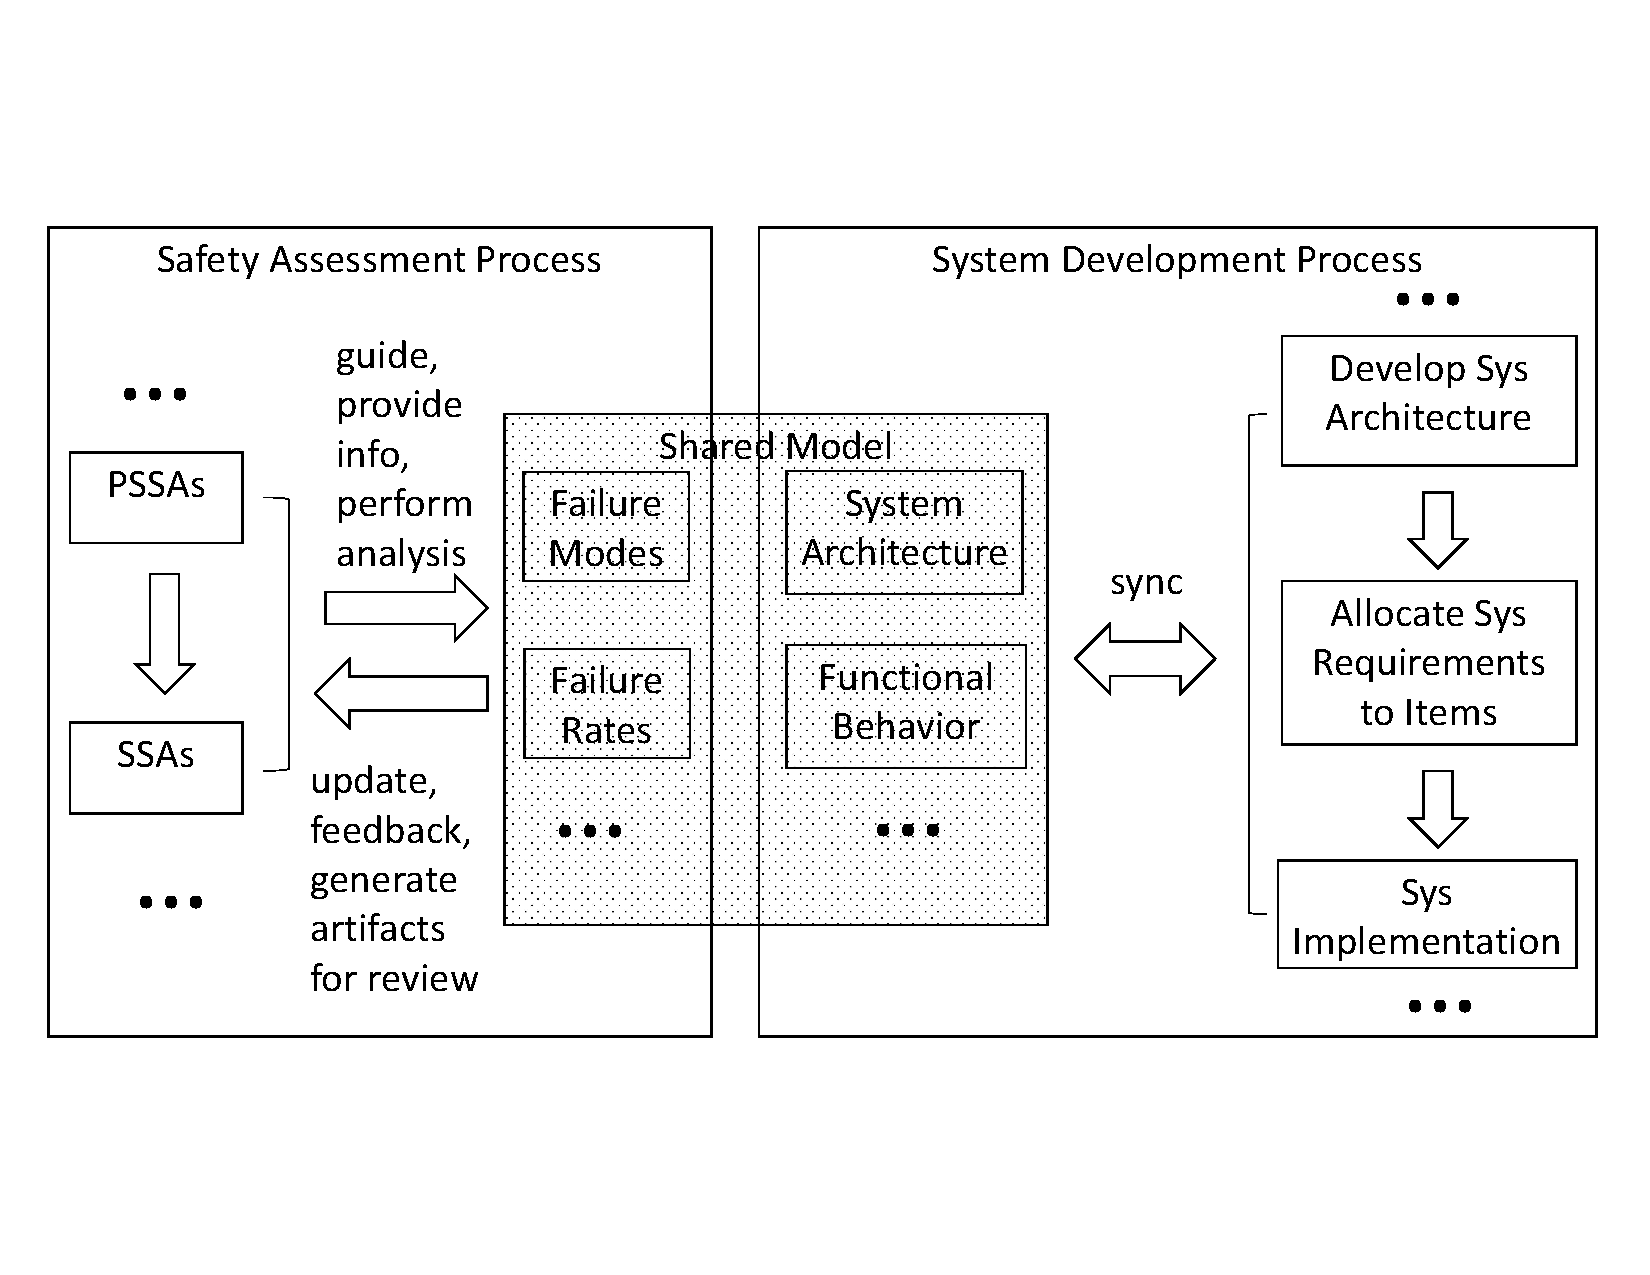
\includegraphics[trim=0 9 0 5,clip,width=0.85\textwidth]{images/safety_process.pdf}
	\vspace{-0.45in}
	\caption{Use of the Shared System/Safety Model in the ARP4754A Safety Assessment Process}
	\label{fig:proposed_safety_process}
\end{figure}

\subsection{Modeling Language for System Design}
\label{subsec:aadl-agree}
%Talk about AADL, AGREE, and why safety annex
%Pull AADL/AGREE background from previous papers to support points in the safety process
%Following the motivation/discussion in the process subsection, talk about why we choose to extend AGREE in safety annex, instead of using a separate safety model, or a semi-separate safety model like EMV2.
The Architectural Analysis and Design Language (AADL)~\cite{FeilerModelBasedEngineering2012} is an SAE International standard~\cite{AADL_Standard} that defines a language and provides a unifying framework for describing the system architecture for ``performance-critical, embedded, real-time systems''~\cite{AADL_Standard}. An AADL model describes a system in terms of a hierarchy of components and their interconnections, where each component can either represent a logical entity (e.g., application software functions, data) or a physical entity (e.g., buses, processors). An AADL model can be associated with properties and be extended with language annexes to provide a richer set of modeling elements for various system design and analysis needs (e.g., performance-related characteristics, configuration settings, dynamic behaviors). The language semantics supports formal analysis tools that allow for early phase error/fault detection.

The Assume Guarantee Reasoning
Environment (AGREE)~\cite{NFM2012:CoGaMiWhLaLu} implements as an AADL annex and annotates AADL components with formal behavioral contracts. Each component's contracts can include assumptions and guarantees about the component's inputs and outputs respectively, as well as predicates on how the state of the component can evolve over time.

AGREE translates an AADL model and the behavioral contracts into Lustre~\cite{Halbwachs91:IEEE} and then query a user-selected
model checker to conduct the back-end verification. The verification is performed compositionally along the architecture hierarchy such that verification at a higher level is only using the components and their behavioral contracts from its immediate lower level. This allows the verification to scale for the design of large and complex systems. 

\begin{comment}
This paper should define how your team of authors see the interaction between "functions" and "system".  
Here is how I see the interaction / relationship:
(a) Aircraft Functions are the highest level
(b) Aircraft Functions are comprised of one or more System
(c) Each System performs one or more System Function
(d) Each System is comprised of one or more LRUs (a.k.a. "items")
\end{comment}

AADL with the AGREE extension serves as a good candidate as the modeling language for describing the system design aspects of a shared system design and safety analysis model. Our prior work~\cite{Stewart17:IMBSA} adds the initial failure effect modeling capability to this language and tool set. However, the following goals are yet to be achieved before the combined language and tool set can be used to satisfy system safety objectives of ARP4754A~\cite{SAE:ARP4754A} and ARP4761~\cite{SAE:ARP4761}:

\begin{enumerate}
	\item Being able to provide a comprehensive, qualitative description of the causal relationship between basic events and system level safety requirements.
	\item Being able to provide an accurate, quantitative description of the contribution relationship between failure rates of the fault tree basic events and numerical probability requirements at the system level.
\end{enumerate}

The remainder of the paper describes our approach towards both of the goals.





\subsection{Example}
\label{subsec:comparison_with_EMV2}

The AADL language has previously been extended to provide some fault modeling and analysis capabilities using its Error Model Annex, Version 2 (EMV2)~\cite{EMV2}.  EMV2 focuses on injection and propagation of discrete faults for generation of fault trees, rather than on analysis of system behavior in the presence of faults. 
To illustrate some of the key differences between our approach and the EMV2 approach, Figure~\ref{fig:comparison_with_EMV2} shows a simplified example based on an aircraft Wheel Brake System (WBS). The WBS model is described in greater detail in ~\cite{Stewart17:IMBSA} and in Section \ref{sec:case_study}. The code fragments in the figure extracted from EMV2, AGREE, and the Safety Annex do not represent the complete code.

In our simplified WBS system, the physical signal from the Pedal component in detected by the Sensor, and the pedal position value is passed to the Braking System Control Unit (BSCU) components.  The BSCU generates a pressure command to the Valve component which applies hydraulic brake pressure to the Wheels. In this example, we use the general term ``fault'' to denote all component errors, hardware failures, and system faults captured by both approaches.

In the EMV2 approach (top half of Figure~\ref{fig:comparison_with_EMV2}), all faults must be explicitly propagated through each component (by applying fault types on each of the output ports) in order for a component to have an impact on the rest of the system. In the example, the ``NoService'' fault is explicitly allowed by the EMV2 declarations to propagate through all of the components.  These fault types are essentially tokens that do not capture any analyzable behavior.  At the system level, analysis tools supporting the EMV2 annex can aggregate the fault flow and propagation information from different components to compose an overall fault flow diagram or fault tree.

In the Safety Annex approach (bottom half of Figure~\ref{fig:comparison_with_EMV2}), faults are captured as faulty behaviors that augment the system behavioral model in AGREE contracts.  When a fault is triggered, the output behavior of the Sensor component is modified, in this case resulting a ``stuck at zero'' error. The behavior of the BSCU receives a zero input and proceeds as if the pedal has not been pressed. This will cause the top level system contract to fail: {\em pedal pressed implies brake pressure output is positive}. No explicit fault propagation is necessary since the faulty behavior itself propagates through the system just as in the nominal system model. The effects of any triggered fault are manifested through analysis of the AGREE contracts. 

\begin{figure}[t]
	\vspace{-0.19in}
	\centering
	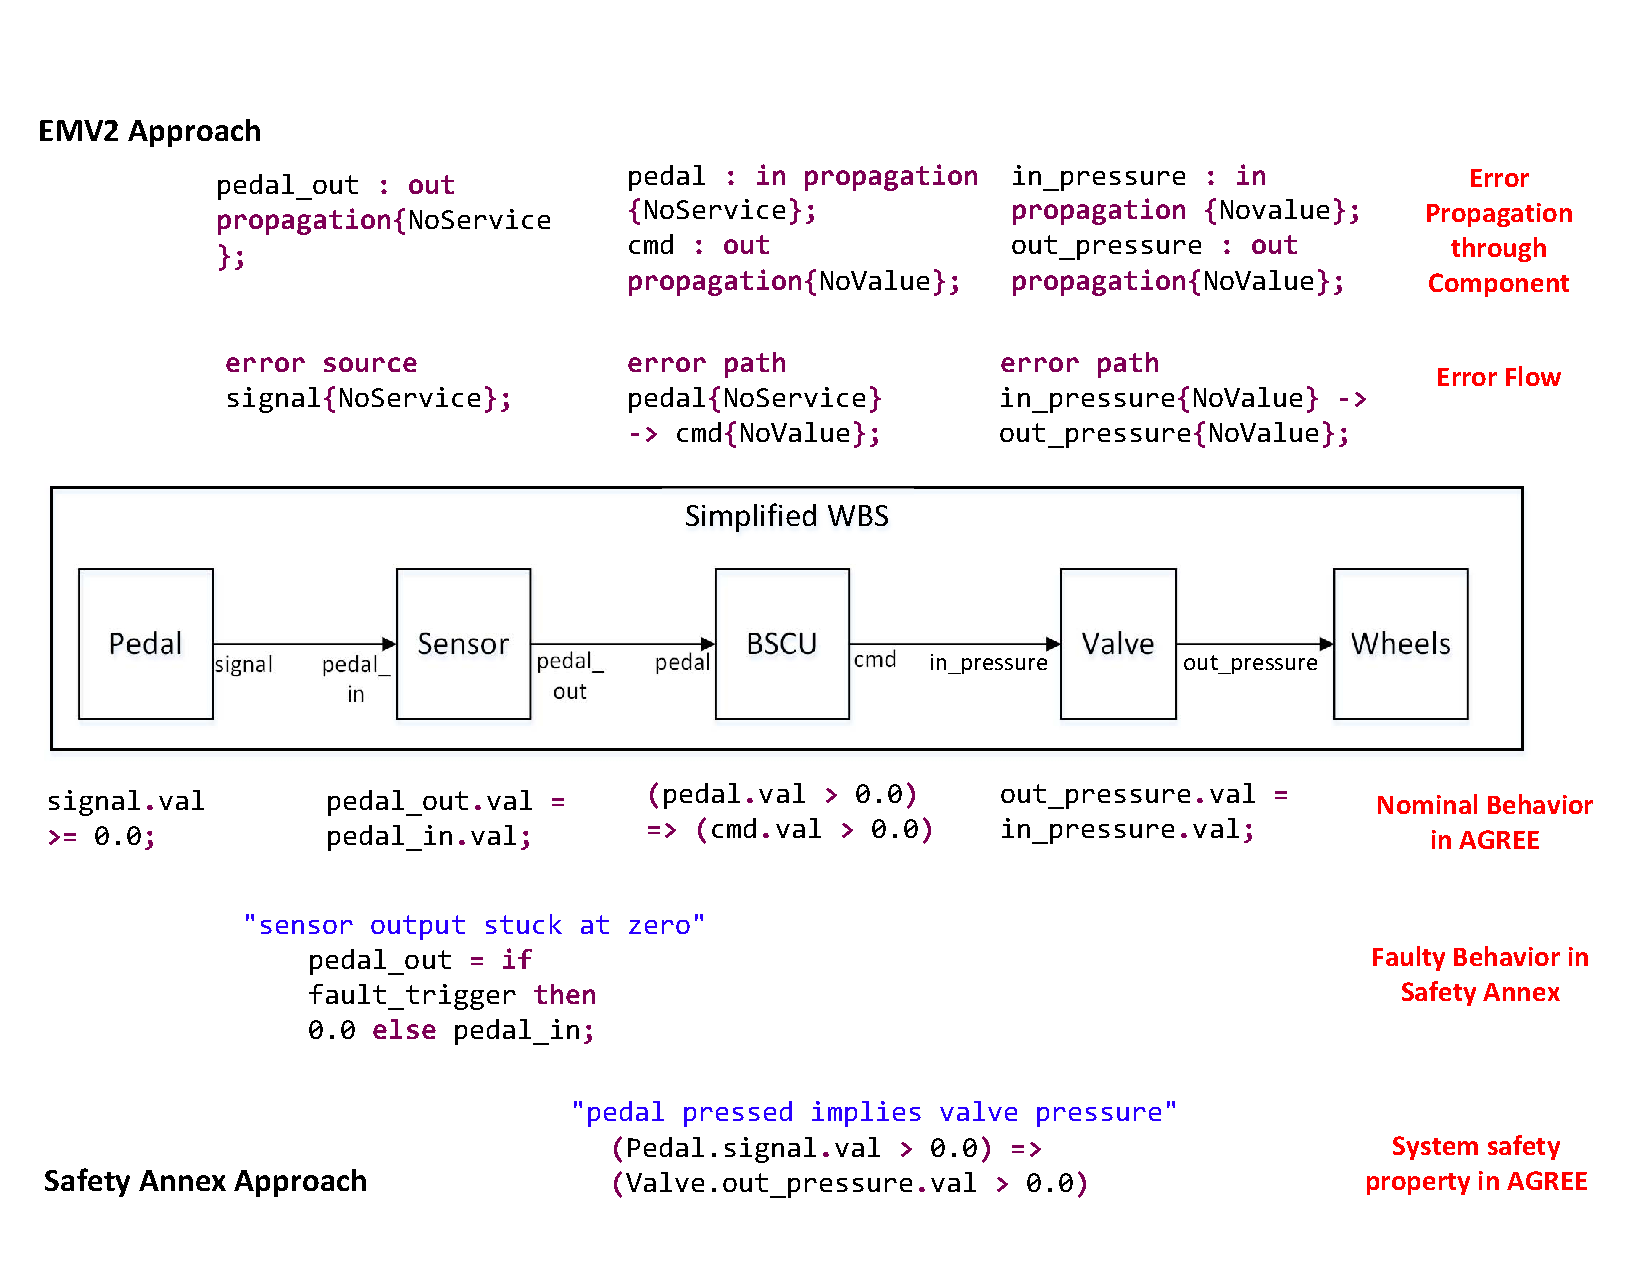
\includegraphics[trim=0 9 0 5,clip,width=\textwidth]{images/Comparison_with_EMV2.pdf}
	%\vspace{0.4in}
	\caption{Differences between Safety Annex and EMV2}
	\label{fig:comparison_with_EMV2}
\end{figure} 
 









\section{Fault Modeling with the Safety Annex}
\label{sec:fault_modeling}

To demonstrate the fault modeling capabilities of the Safety Annex we will use the Wheel Brake System (WBS) described in AIR6110~\cite{AIR6110}.  This system is a well-known example that has been used as a case study for safety analysis, formal verification, and contract based design~\cite{DBLP:conf/cav/BozzanoCPJKPRT15, 10.1007/978-3-319-11936-6-7, CAV2015:BoCiGrMa, Joshi05:SafeComp}. %The preliminary work for the safety annex was based on a simple model of the WBS~\cite{Stewart17:IMBSA}. To demonstrate a more complex fault modeling process, we constructed a functionally and structurally equivalent AADL version of one of the more complex WBS NuSMV/xSAP model (arch4wbs)~\cite{DBLP:conf/cav/BozzanoCPJKPRT15}.    

\begin{figure}[h!]
	\centering
	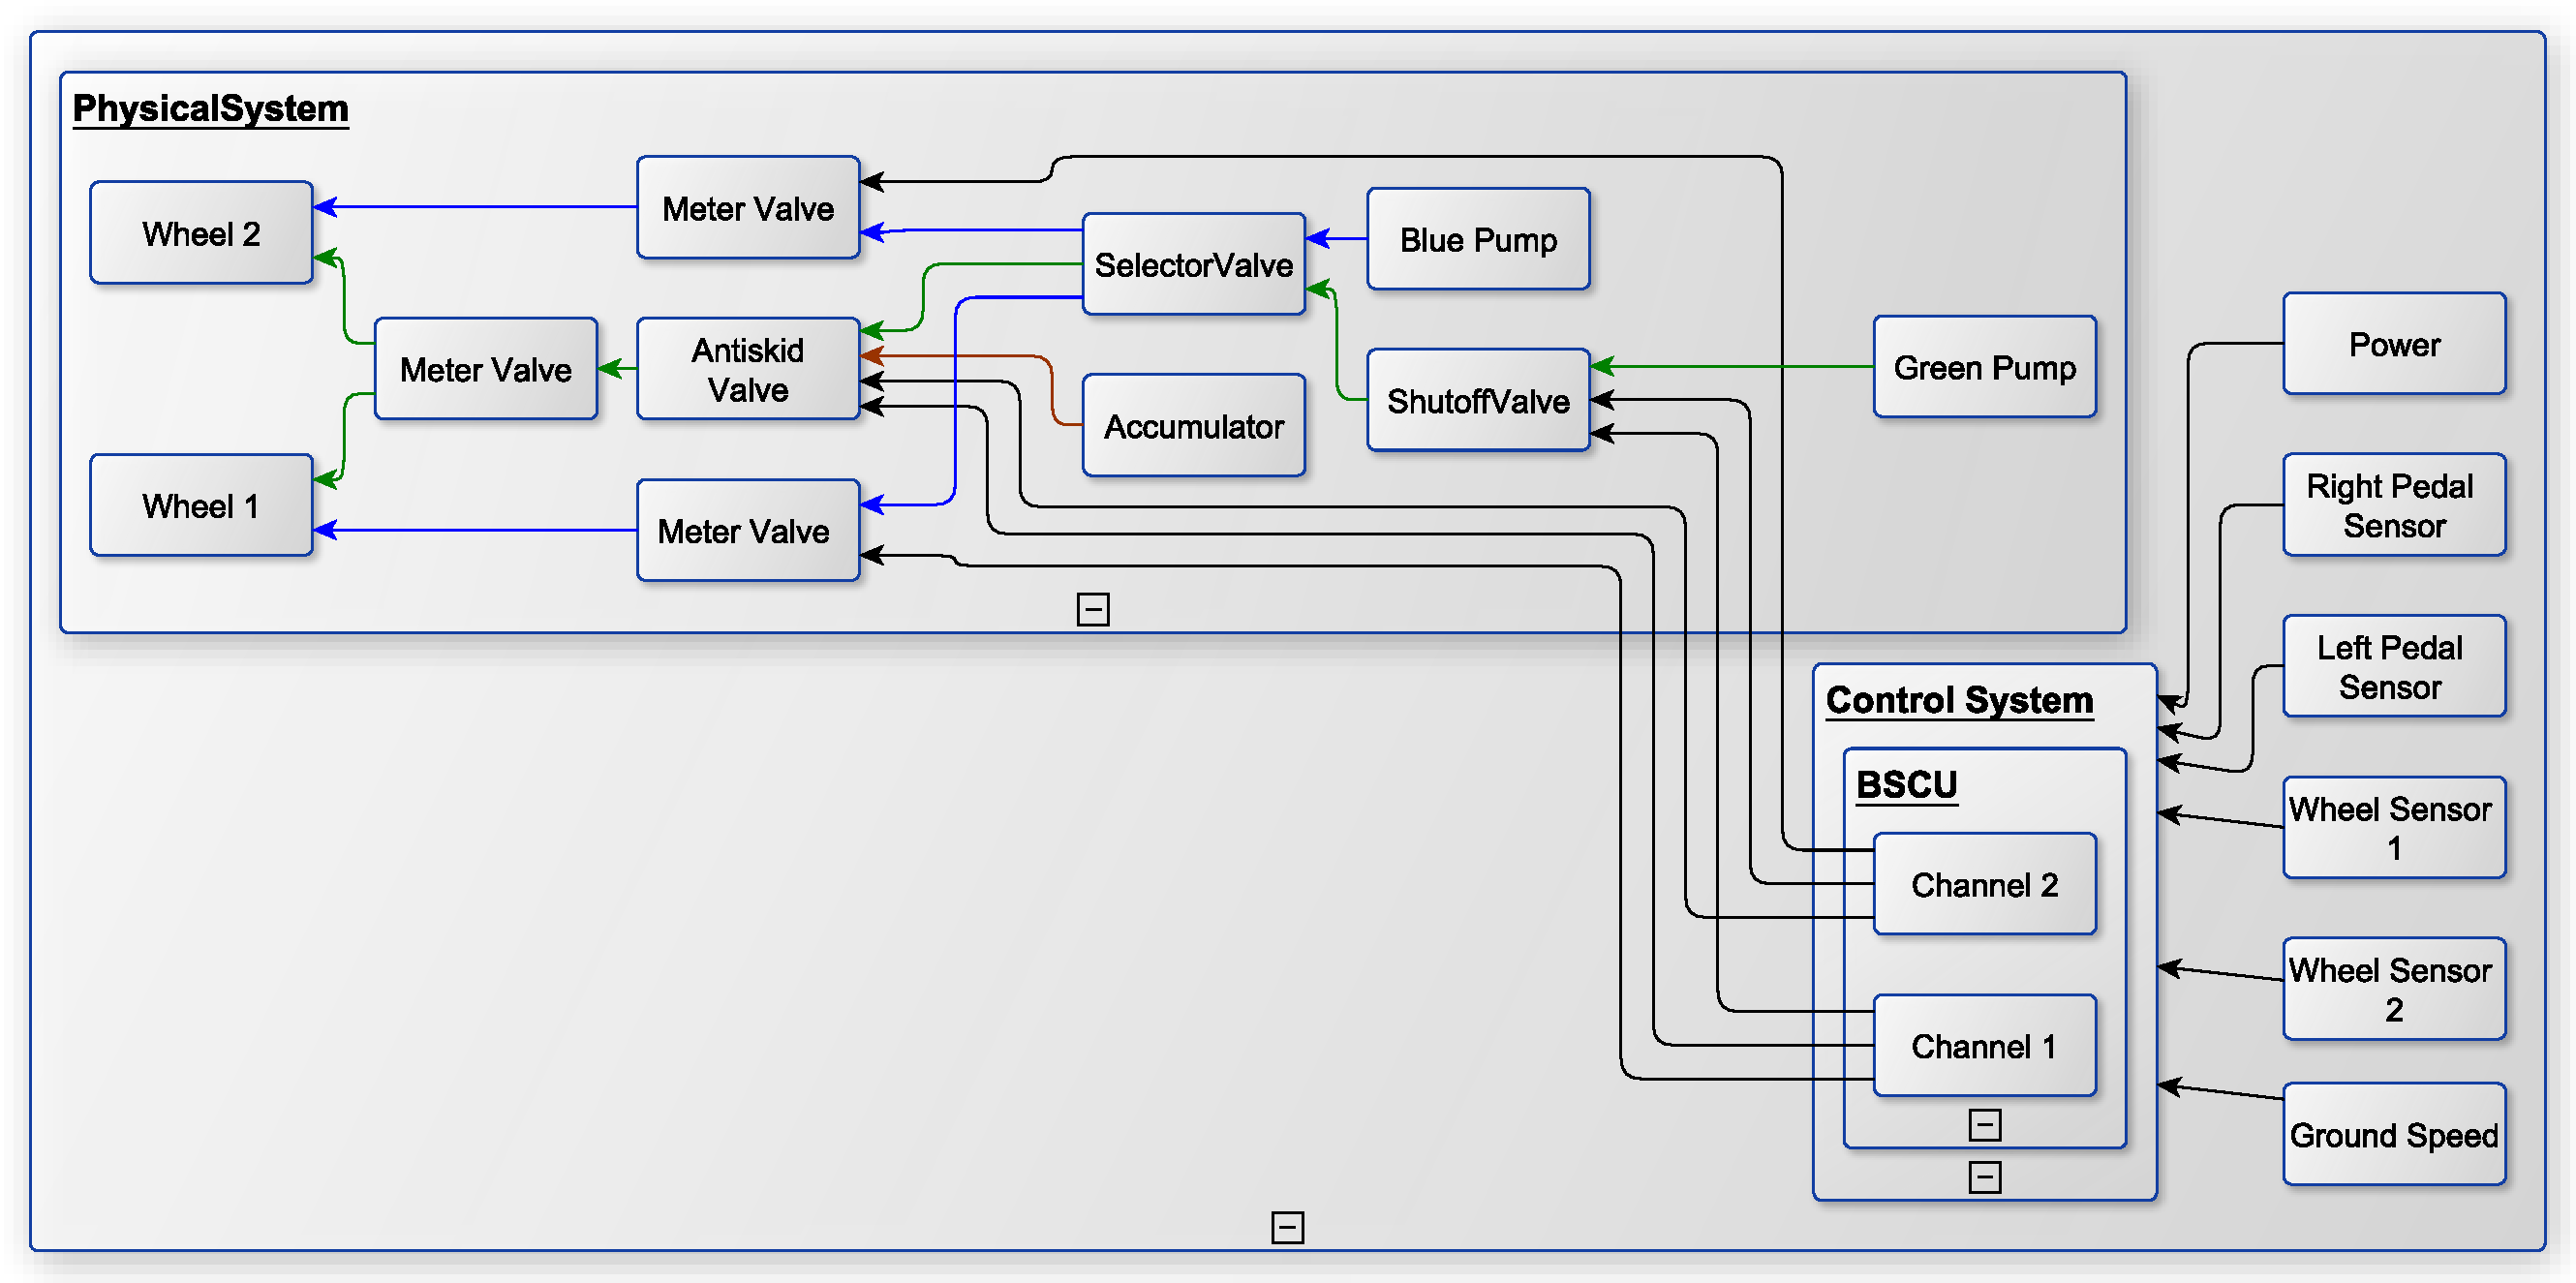
\includegraphics[trim=0 9 0 5,clip,width=\textwidth]{images/wbs_arch4_diagram.pdf}
	\caption{Wheel Brake System}
	\label{fig:wbs}
\end{figure} 

The WBS is composed of two main parts: the control system and the physical system. The control system electronically controls the physical system and contains a redundant channel of the Braking System Control Unit (BSCU) in case of failure. It also commands antiskid braking.% in case of skidding on the ground. 
The physical system consists of the hydraulic circuits running from hydraulic pumps to wheel brakes as well as valves that control the hydraulic fluid flow. This system provides braking force to each of the eight wheels of the aircraft. The wheels are all mechanically braked in pairs (one pair per landing gear). For simplicity, Figure~\ref{fig:wbs} displays only two of the eight wheels. 

There are three operating modes in the WBS model:

\begin{itemize}
	\renewcommand{\labelitemi}{\textbullet}
	\item In \textit{normal} mode, the system is composed of a \textit{green} hydraulic pump and one meter valve per each of the eight wheels. Each of the meter valves are controlled through electronic commands coming from the active channel of the BSCU. These signals provide braking and antiskid commands for each wheel. The braking command is determined through a sensor on the pedal and the antiskid command is determined by the \textit{Wheel Sensors}. 
	\item In \textit{alternate} mode, the system is composed of a \textit{blue} hydraulic pump, four meter valves, and four antiskid shutoff valves, one for each landing gear. The meter valves are mechanically commanded through the pilot pedal corresponding to each landing gear. If the system detects lack of pressure in the green circuit, the BSCU channel commands the selector valve to switch to the blue circuit. 
	\item In \textit{emergency} mode, the system mode is entered if the \textit{blue} hydraulic pump fails. The accumulator pump has a reserve of pressurized hydraulic fluid and will supply this to the blue circuit in emergency mode. 
\end{itemize}

The WBS architecture model in AADL contains 30 different kinds of components, 169 component instances, and a model depth of 5 hierarchical levels. 


%If the BSCU channel becomes invalid, the shutoff valve closes and we move into alternate mode. Once this system switches into alternate mode, it does not return to normal operation mode.

%There are three operating modes in the WBS model. In \textit{normal} mode, the system uses the \textit{green} hydraulic circuit. The normal system is composed of the green hydraulic pump and one meter valve per each of the eight wheels. Each of the meter valves are controlled through electronic commands coming from the active channel of the BSCU. These signals provide braking and antiskid commands for each wheel. The braking command is determined through a sensor on the pilot pedal position and is labeled as \textit{Left/Right Pedal Sensor} in Figure~\ref{fig:wbs} and the antiskid command is determined by the \textit{Wheel Sensors}. 

%In \textit{alternate} mode, the system uses the \textit{blue} hydraulic circuit. The alternate system is composed of the blue hydraulic pump, four meter valves, and four antiskid shutoff valves: one for each landing gear. The meter valves are mechanically commanded through the pilot pedal corresponding to each landing gear. If the system detects lack of pressure in the green circuit, the BSCU channel commands the selector valve to switch to the blue circuit. 
%If the BSCU channel becomes invalid, the shutoff valve closes and we move into alternate mode. Once this system switches into alternate mode, it does not return to normal operation mode.

%The last mode of operation of the WBS is the \textit{emergency} mode. This mode is entered if the blue hydraulic pump fails. The accumulator pump has a reserve of pressurized hydraulic fluid and will supply this to the blue circuit in emergency mode.

%The model contains 30 different kinds of components, 169 component instances, a model depth of 5 hierarchical levels.  The model includes one top-level assumption and  11 top-level system properties, with 113 guarantees allocated to subsystems.  There are a total of 33 different fault types and 141 fault instances within the model.  The large number of fault instances is due to the redundancy in the system design and its replication to control 8 wheels.

The behavioral model is encoded using the AGREE annex and the behavior is based on descriptions found in AIR6110. The top level system properties are given by the requirements and safety objectives in AIR6110. All of the subcomponent contracts support these system safety objectives through the use of assumptions on component input and guarantees on the output. The WBS behavioral model in AGREE annex includes one top-level assumption and  11 top-level system properties, with 113 guarantees allocated to subsystems.  

An example system safety property is to ensure that there is no inadvertent braking of any of the wheels. This is based on a failure condition described in AIR6110 is \textit{Inadvertent wheel braking on one wheel during takeoff shall be less than 1E-9 per takeoff}. 
Inadvertent braking means that braking force is applied at the wheel but the pilot has not pressed the brake pedal.  In addition, the inadvertent braking requires that power and hydraulic pressure are both present, the plane is not stopped, and the wheel is rolling (not skidding). 
%in Figure~\ref{fig:inadvertent_braking}. 
The property is stated in AGREE such that inadvertent braking does \textit{not} occur, as shown below. 

\begin{figure}[h!]
	\vspace{-0.2in}
	\begin{center}
		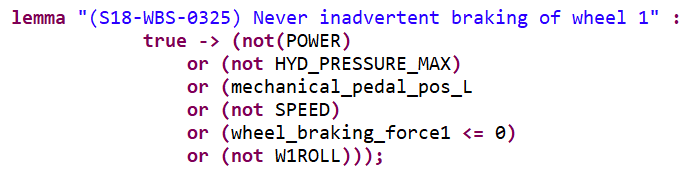
\includegraphics[width=.8\textwidth]{images/inadvertent_braking.png}
	\end{center}
	\vspace{-0.3in}
	%\caption{AGREE Contract for Top Level Property}
	\label{fig:inadvertent_braking}
	\vspace{-0.2in}
\end{figure}


\subsection{Component Fault Modeling}

The usage of the terms error, failure, and fault are defined in ARP4754A and are described here for ease of understanding~\cite{SAE:ARP4754A}. An \textit{error} is a mistake made in implementation, design, or requirements. A \textit{fault} is the manifestation of an error and a \textit{failure} is an event that occurs when the delivered service of a system deviates from correct behavior. If a fault is activated under the right circumstances, that fault can lead to a failure. The terminology used in EMV2 differs slightly for an error: an error is a corrupted state caused by a fault. The error propagates through a system and can  manifest as a failure. In this paper, we use the ARP4754A terminology with the added definition of \textit{error propagation} as used in EMV2. An error is a mistake made in design or code and an error propagation is the corrupted state caused by an active fault. 

The Safety Annex is used to add potential faulty behaviors to a component model.  When the fault is activated by its specified triggering conditions, it modifies the output of the component. This faulty behavior may violate the contracts of other components in the system, including assumptions of downstream components. The impact of a fault is computed by the AGREE model checker when the safety analysis is run on the fault model. Examples of such faults include valves being stuck open or closed, output of a software component being nondeterministic, or power being cut off. 
%Faulty components can be mechanical or digital, but in this section we focus on a digital component in the WBS -- a brake pedal position sensor component. 

One of the components important to the inadvertent braking property is the brake pedal. When the mechanical pedal is pressed, a sensor reads this information and passes an electronic signal to the BSCU which then commands hydraulic pressure to the wheels. 

%Figure~\ref{fig:sensor} 
Below shows the AADL pedal sensor component with a contract for its nominal behavior. The sensor has only one input, the mechanical pedal position, and one output, the electrical pedal position. %The 
A property that governs the behavior of the component is that the mechanical position should always equal the electronic position. 

\begin{figure}[h!]
	\hspace*{-2cm}
	\vspace{-0.55in} 
	\begin{center}
		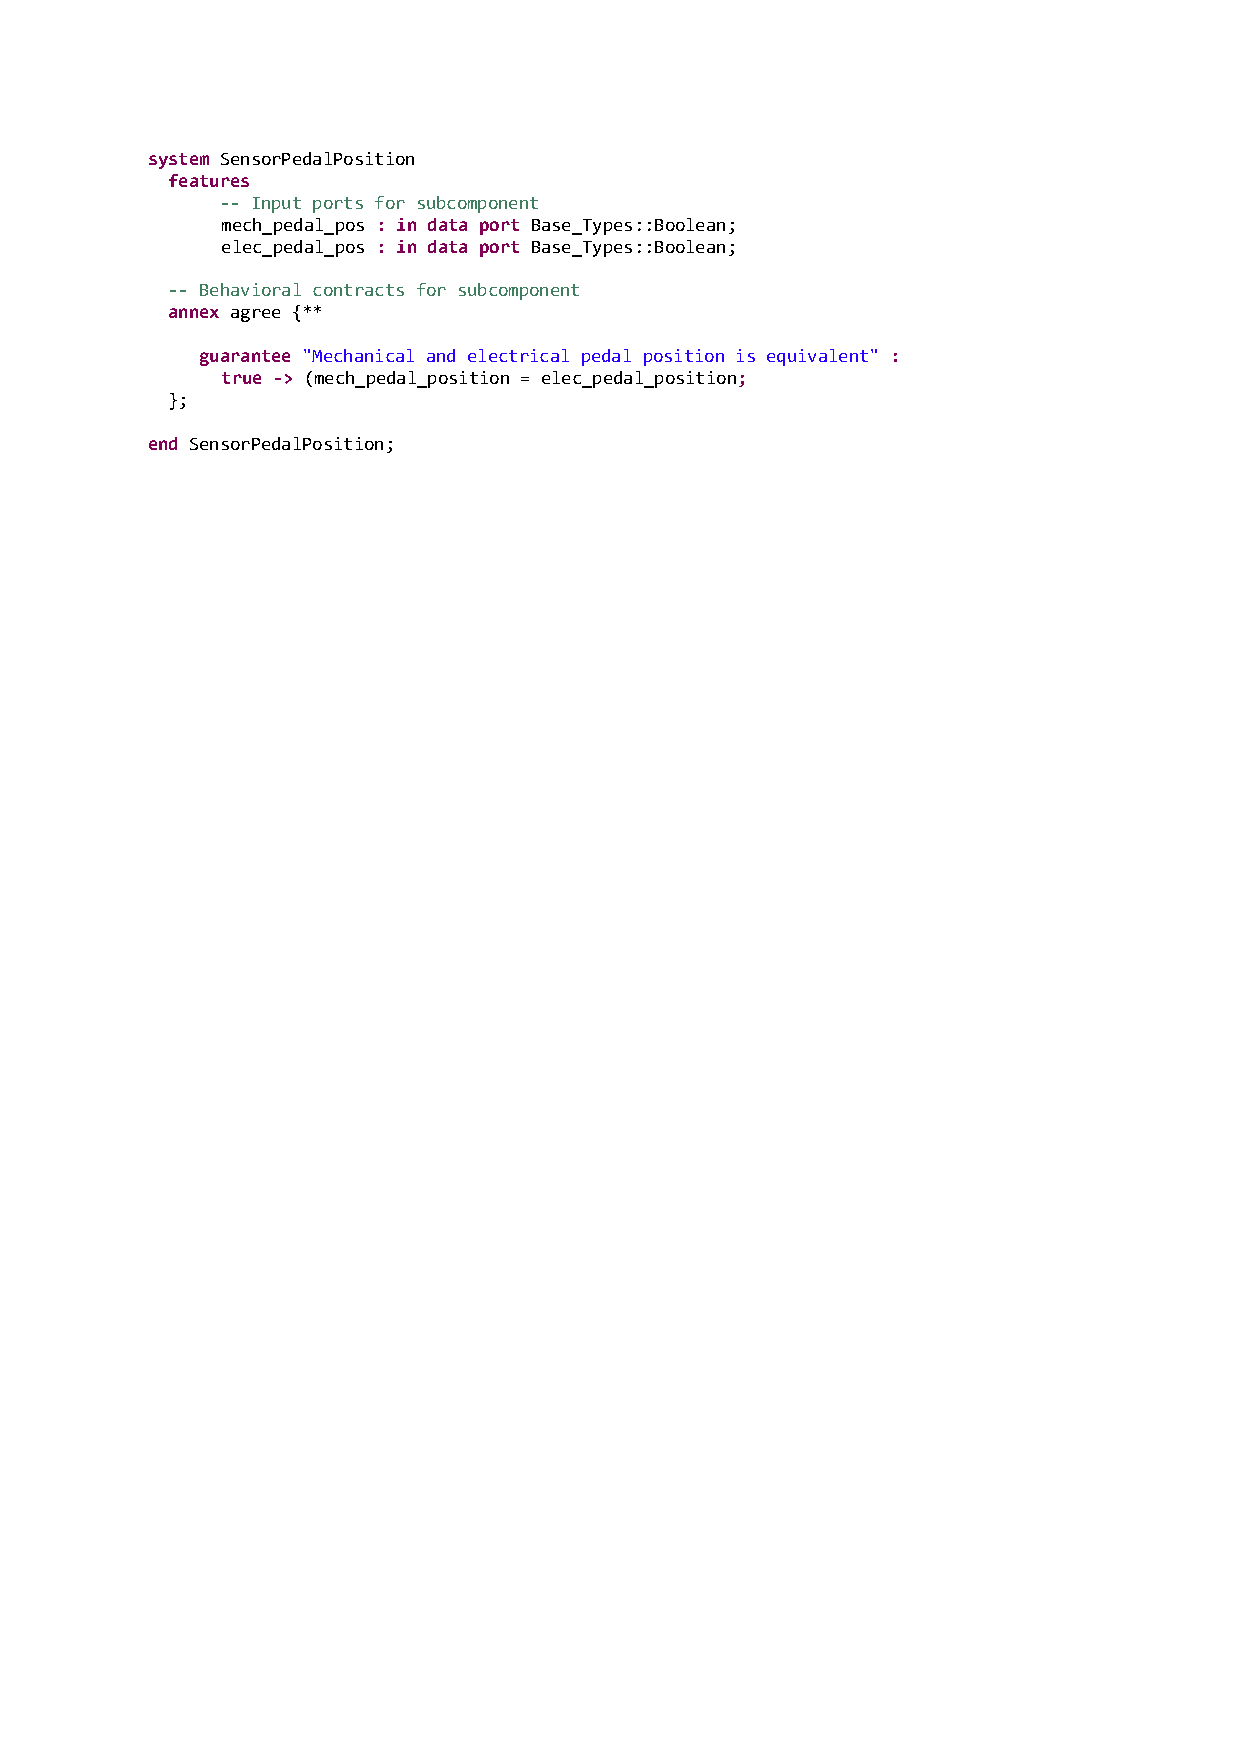
\includegraphics[trim=0 640 -10 70,clip,width=1.5\dimexpr\textwidth-2cm\relax]{images/system_sensor.pdf}
		\vspace{-0.3in}
	%	\caption{An AADL System Type: The Pedal Sensor}
		\label{fig:sensor}
	\end{center}
	\vspace{-0.4in}
\end{figure}

One possible failure for this sensor is inversion of its output value. This fault can be triggered with probability $5.0\times 10^{-6}$ as described in AIR6110 (in reality, the component failure probability is 
collected from hardware specification sheets).  %Figure~\ref{fig:sensorFault} 
The Safety Annex definition for this fault is shown below. Fault behaviors may be defined by the user or by using a library of fault nodes, in this case, \textit{inverted\_fail}.  When the fault is triggered, the nominal output of the component (\textit{elec\_pedal\_position}) is replaced with its failure value (\textit{val\_out}). 

\begin{figure}[h!]
	\hspace*{-2cm}
	\vspace{-0.5in} 
	\begin{center}
		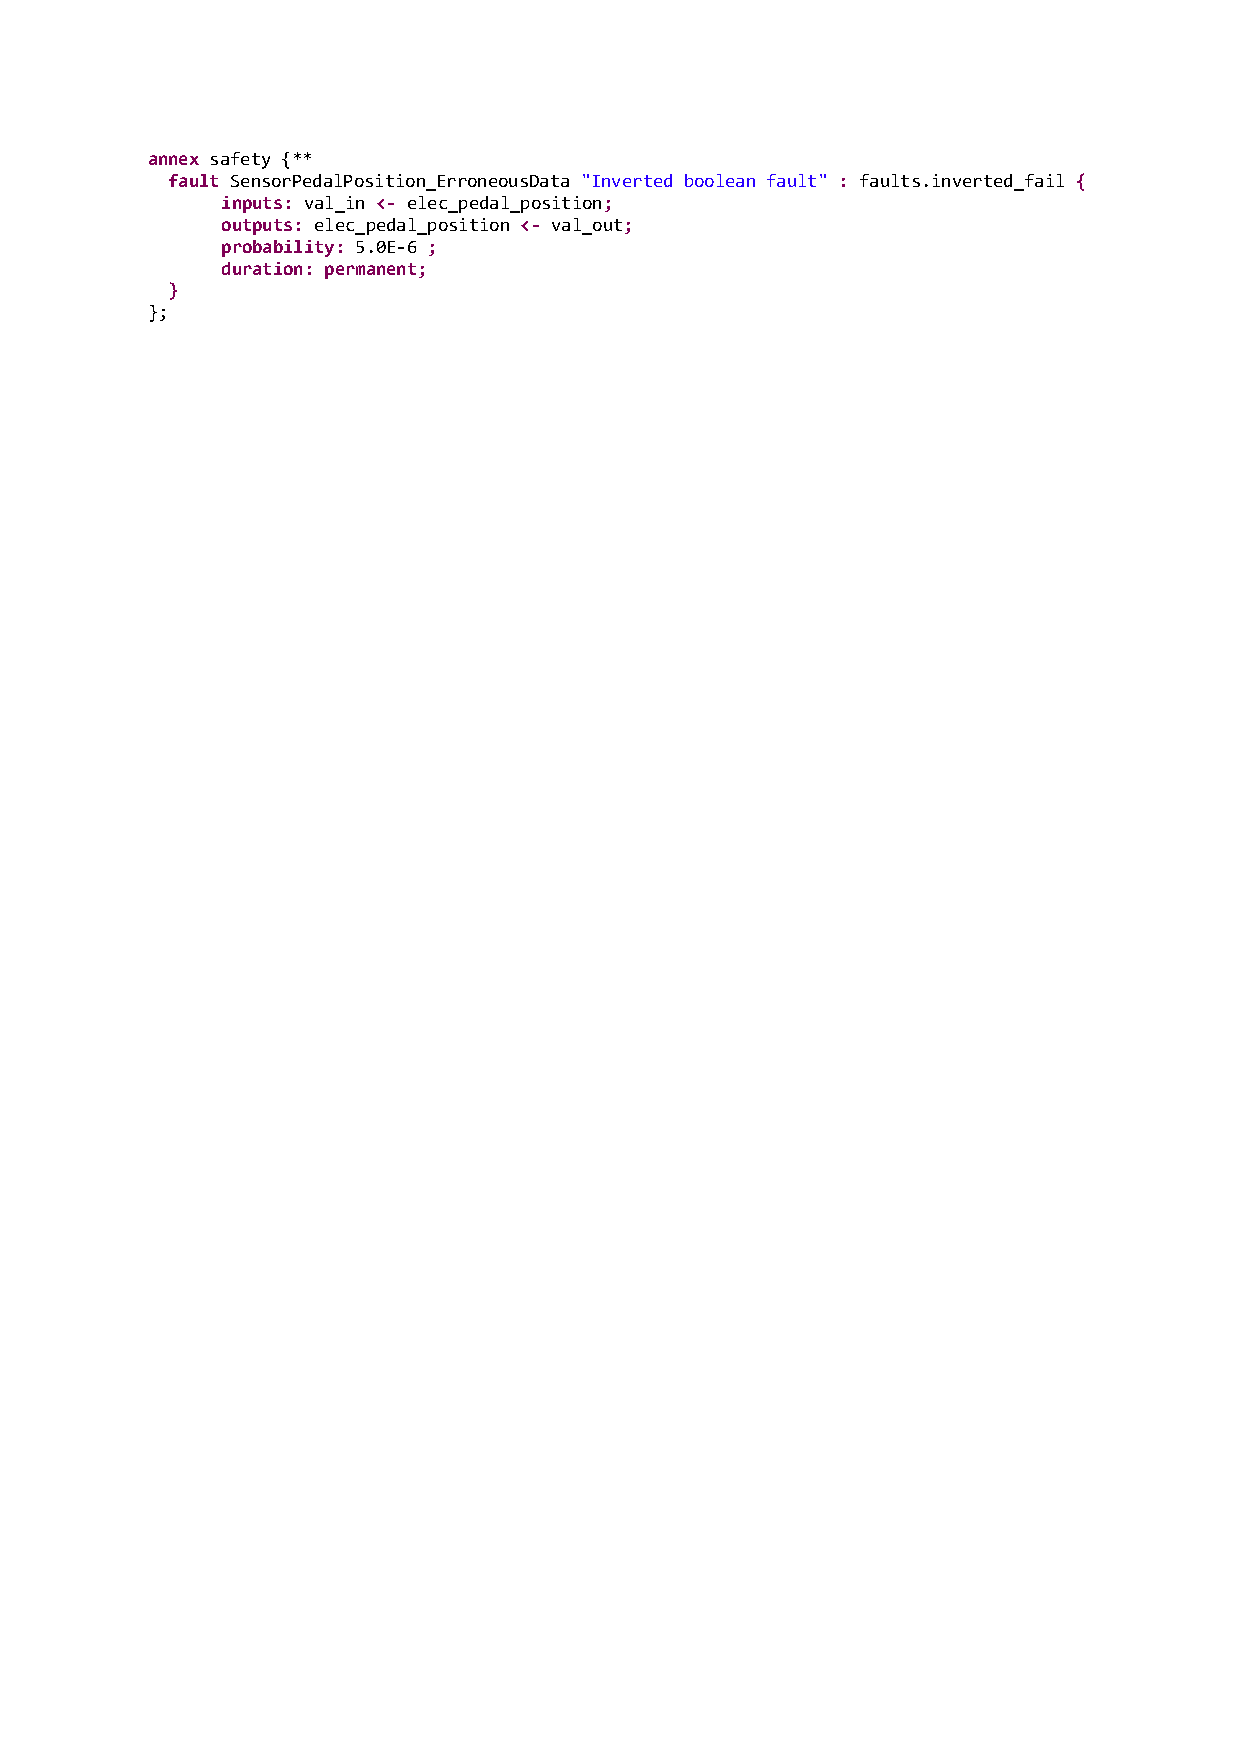
\includegraphics[trim=0 690 -10 70,clip,width=1.5\dimexpr\textwidth-2cm\relax]{images/safetyannex_sensorfault.pdf}
		\vspace{-0.3in}
		%\caption{The Safety Annex for the Pedal Sensor}
		\label{fig:sensorFault}
	\end{center}
	\vspace{-0.3in}
\end{figure}

The WBS fault model in Safety Annex contains a total of 33 different fault types and 141 fault instances. The large number of fault instances is due to the redundancy in the system design and its replication to control 8 wheels.

\subsection{Implicit %Failure
	Error Propagation}
In the Safety Annex approach, faults are captured as faulty behaviors that augment the system behavioral model in AGREE contracts. No explicit %fault
error propagation is necessary since the faulty behavior itself propagates through the system just as in the nominal system model. The effects of any triggered fault are manifested through analysis of the AGREE contracts. 

On the contrary, in the AADL Error Model Annex, Version 2 (EMV2)~\cite{EMV2} approach, all errors must be explicitly propagated through each component (by applying fault types on each of the output ports) in order for a component to have an impact on the rest of the system. To illustrate the key differences between implicit %failure
error propagation provided in Safety Annex and the explicit %failure 
error propagation provided in EMV2, we use a simplified behavioral flow from the WBS example using code fragments from EMV2, AGREE, and the Safety Annex. 

\begin{figure}[t]
	\vspace{-0.19in}
	\centering
	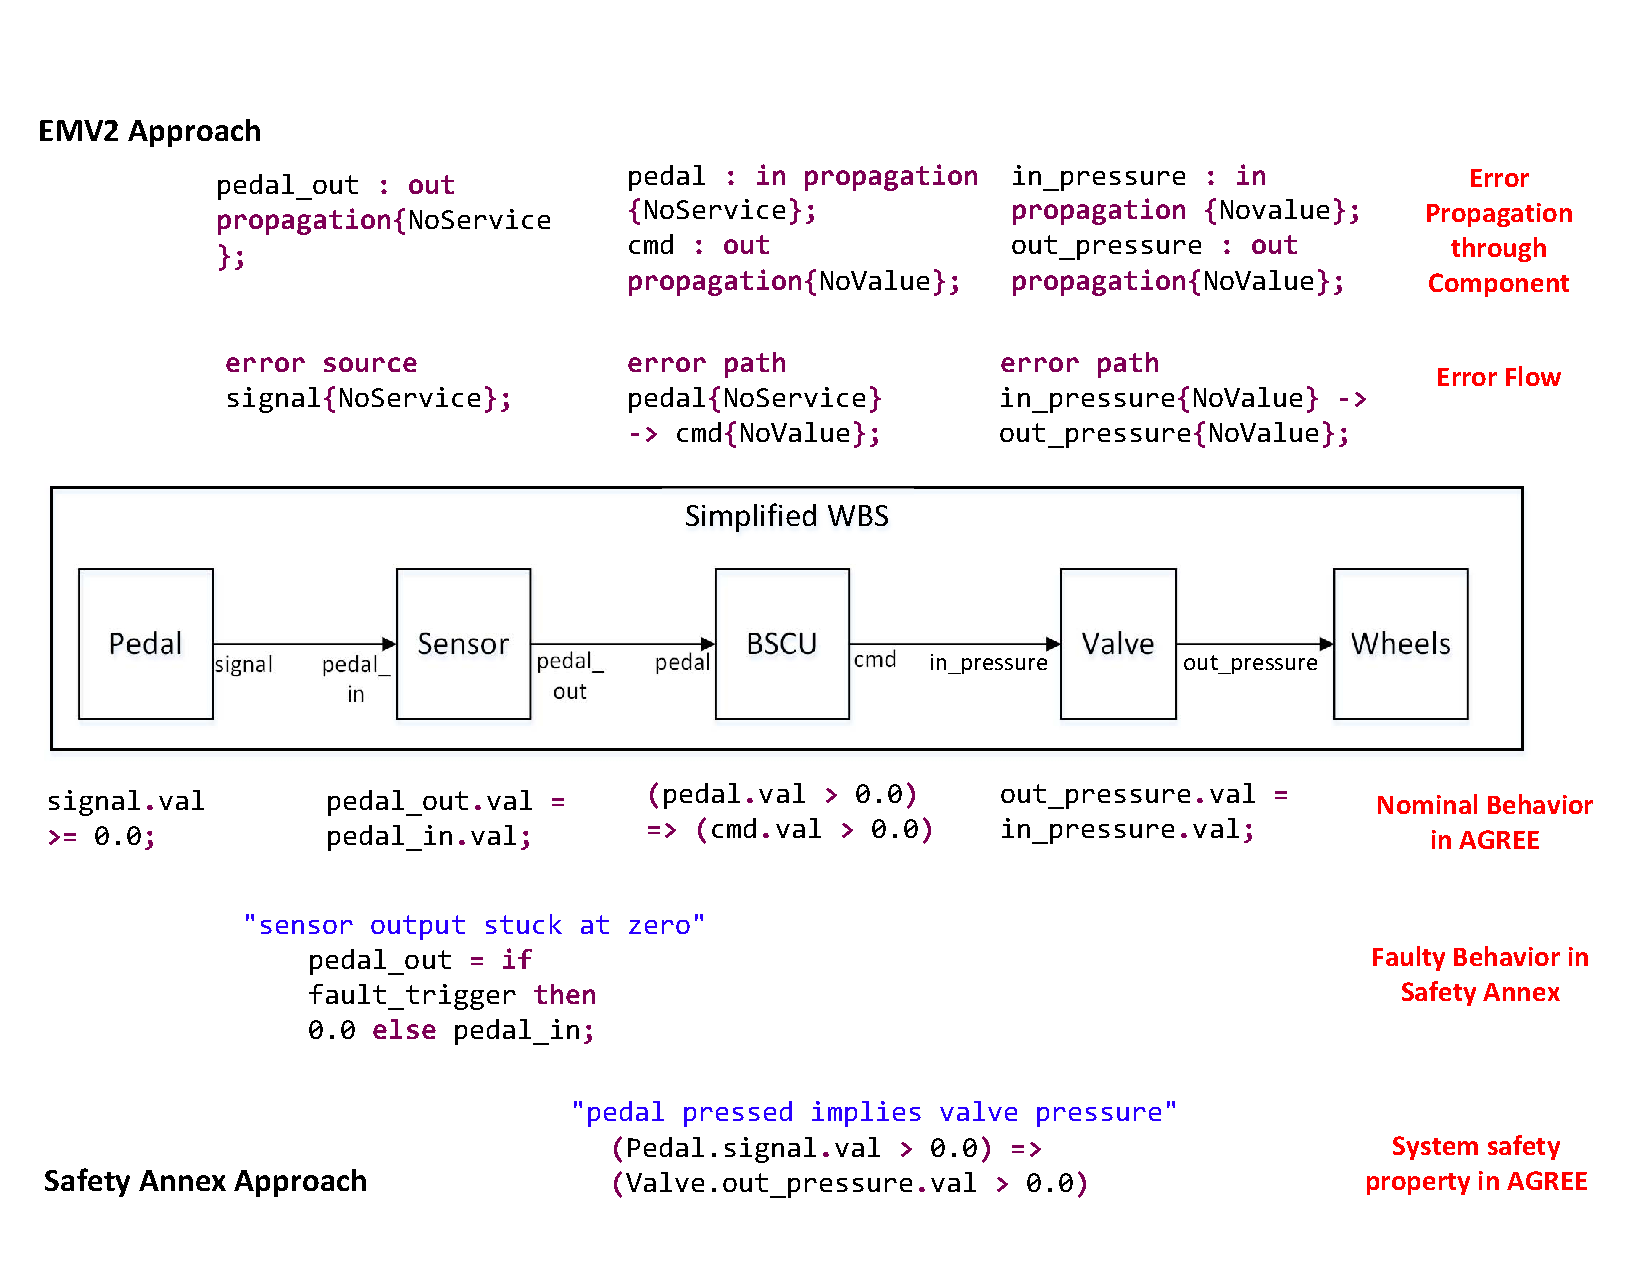
\includegraphics[trim=0 9 0 5,clip,width=\textwidth]{images/Comparison_with_EMV2.pdf}
	\vspace{-0.3in}
	\caption{Differences between Safety Annex and EMV2}
	\label{fig:comparison_with_EMV2}
	\vspace{-0.2in}
\end{figure} 

In this simplified WBS system, the physical signal from the Pedal component is detected by the Sensor and the pedal position value is passed to the Braking System Control Unit (BSCU) components.  The BSCU generates a pressure command to the Valve component which applies hydraulic brake pressure to the Wheels. 

In the EMV2 approach (top half of Figure~\ref{fig:comparison_with_EMV2}), the ``NoService'' fault is explicitly propagated through all of the components. These fault types are essentially tokens that do not capture any analyzable behavior. At the system level, analysis tools supporting the EMV2 annex can aggregate the propagation information from different components to compose an overall fault flow diagram or fault tree. 

When a fault is triggered in the Safety Annex (bottom half of Figure~\ref{fig:comparison_with_EMV2}), the output behavior of the Sensor component is modified. In this case the result is a ``stuck at zero'' error. The behavior of the BSCU receives a zero input and proceeds as if the pedal has not been pressed. This will cause the top level system contract to fail: {\em pedal pressed implies brake pressure output is positive}.

\begin{comment}
%\subsection{Comparison to the AADL Error Annex}

The AADL language has previously been extended to provide some fault modeling and analysis capabilities using its Error Model Annex, Version 2 (EMV2)~\cite{EMV2}.  EMV2 focuses on injection and propagation of discrete faults for generation of fault trees, rather than on analysis of system behavior in the presence of faults. 
To illustrate some of the key differences between our approach and the EMV2 approach, Figure~\ref{fig:comparison_with_EMV2} shows a simplified  behavioral flow with code fragments from EMV2, AGREE, and the Safety Annex. 

\begin{figure}[t]
	\vspace{-0.45in}
	\centering
	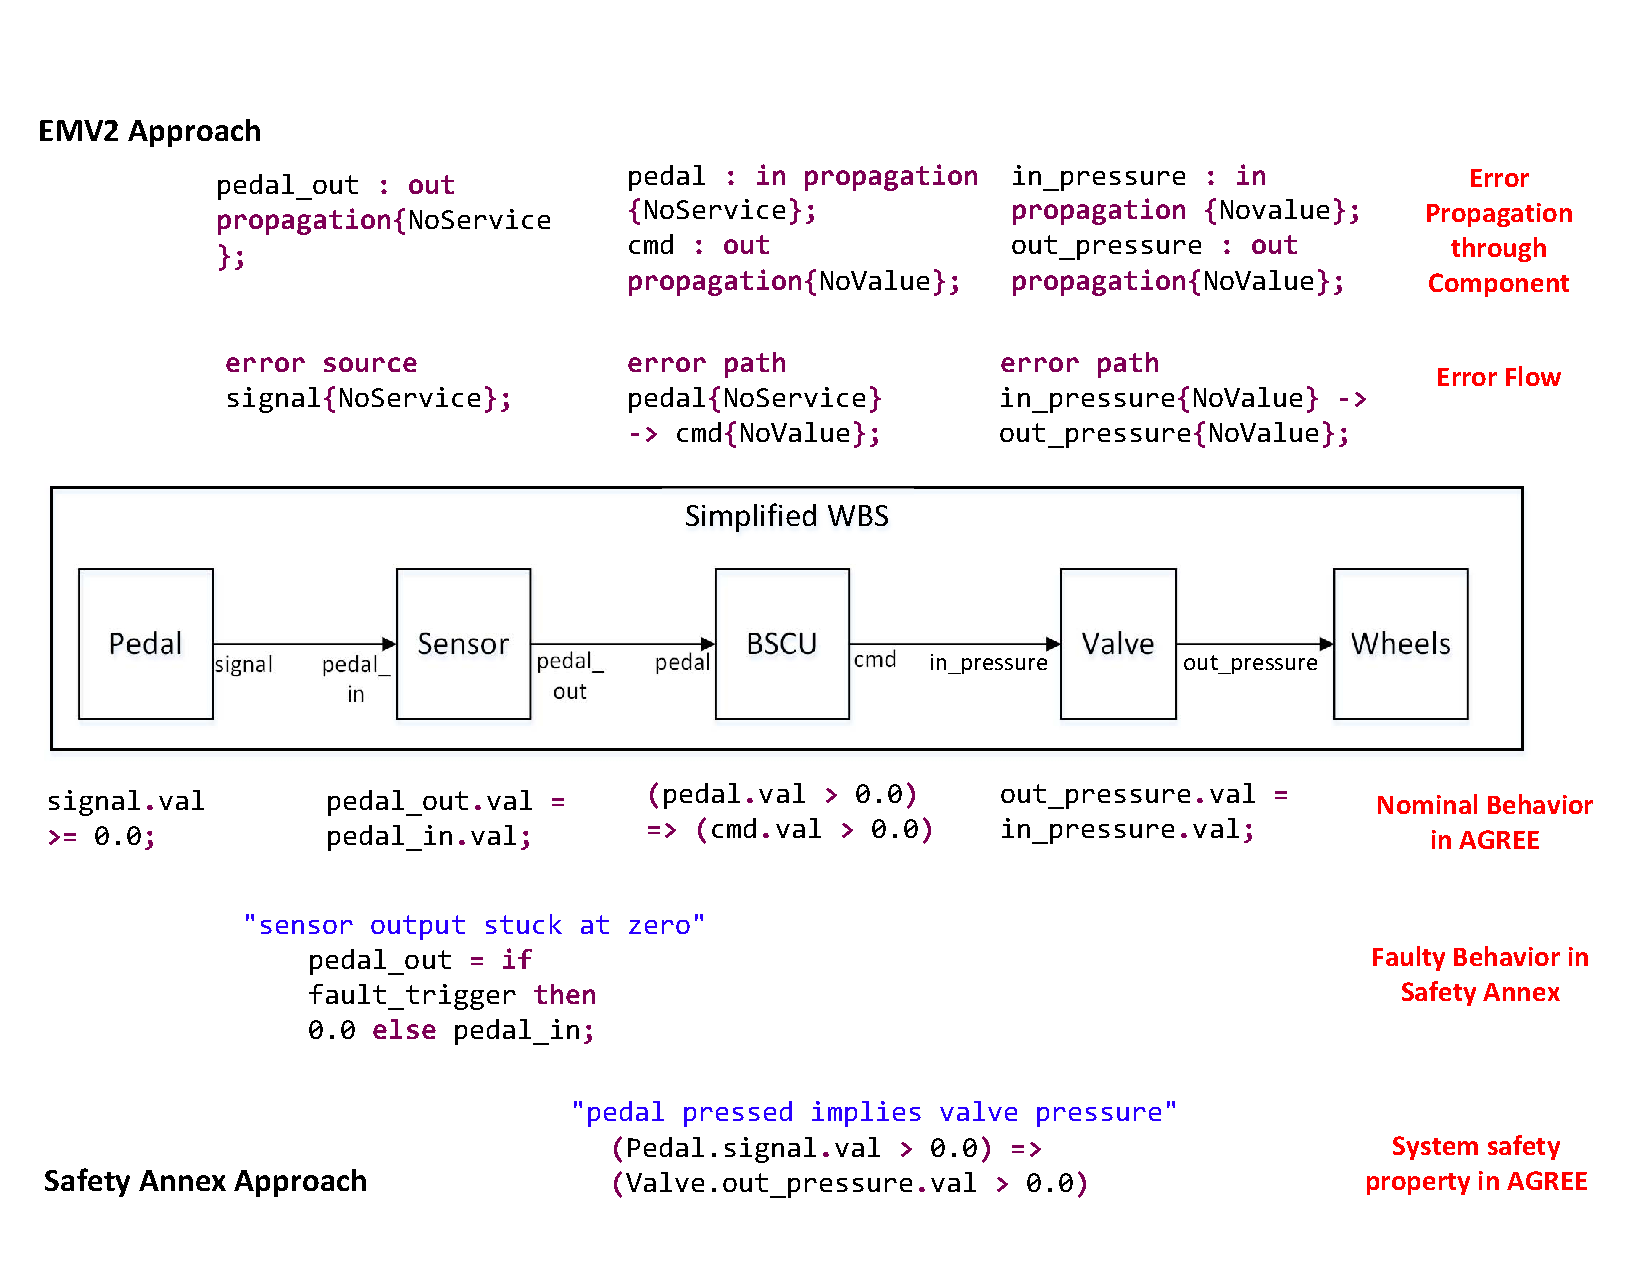
\includegraphics[trim=0 9 0 5,clip,width=\textwidth]{images/Comparison_with_EMV2.pdf}
	%\vspace{0.4in}
	\caption{Differences between Safety Annex and EMV2}
	\label{fig:comparison_with_EMV2}
\end{figure} 

In this simplified WBS system, the physical signal from the Pedal component is detected by the Sensor, and the pedal position value is passed to the Braking System Control Unit (BSCU) components.  The BSCU generates a pressure command to the Valve component which applies hydraulic brake pressure to the Wheels. 

In the EMV2 approach (top half of Figure~\ref{fig:comparison_with_EMV2}), all errors must be explicitly propagated through each component (by applying fault types on each of the output ports) in order for a component to have an impact on the rest of the system. In the example, the ``NoService'' fault is explicitly allowed by the EMV2 declarations to propagate through all of the components.  These fault types are essentially tokens that do not capture any analyzable behavior.  At the system level, analysis tools supporting the EMV2 annex can aggregate the fault flow and propagation information from different components to compose an overall fault flow diagram or fault tree.

In the Safety Annex approach (bottom half of Figure~\ref{fig:comparison_with_EMV2}), faults augment the system behavioral model through the AGREE contracts.  When a fault is triggered, the output behavior of the Sensor component is modified, in this case resulting a ``stuck at zero'' error. The behavior of the BSCU receives a zero input and proceeds as if the pedal has not been pressed. This will cause the top level system contract to fail: {\em pedal pressed implies brake pressure output is positive}. No explicit propagation is necessary since the faulty behavior propagates through the system just as in the nominal system model. The system and component failures are manifested through analysis of the AGREE contracts. 
\end{comment}

\subsection{Explicit %Failure 
	Error Propagation} 
%Faults
Failures in hardware (HW) components can trigger behavioral faults in the system components that depend on them. For example, a CPU %fault
Failure may trigger faulty behavior in the threads bound to that CPU. In addition, a %fault
failure in one HW component may trigger %faults
failure in other HW components located nearby, such as overheating, fire, or explosion
in the containment location. 
The Safety Annex provides the capability to explicitly model the impact of hardware %faults
failures on other faults, behavioral or non behavioral. The explicit propagation to non behavioral faults is similar to that provided in EMV2.

To better model %HW dependent faults 
faults at the system level dependent on HW failures, a fault model element is introduced called a \textit{hardware fault}. Users are not required to specify behavioral effects for the HW faults, nor are data ports necessary on which to apply the fault definition. An example of a model component fault declaration is shown below:
\begin{figure}[h!]
	\vspace{-0.2in}
	\begin{center}
	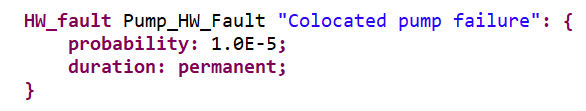
\includegraphics[width=.7\textwidth]{images/hw_fault2.png}
	\end{center}
	\vspace{-0.3in}
	%\caption{Hardware Fault Definition}
	\label{fig:hwFault}
	%\vspace{-0.2in}
	\vspace{-0.1in}
\end{figure}

Users specify dependencies between the HW component faults and faults that are defined in other components, either HW or SW. The hardware fault then acts as a trigger for dependent faults. This allows a simple propagation from the faulty HW component to the SW components that rely on it, affecting the behavior on the outputs of the affected SW components.

%As an example, we will look yet again at the WBS. 
In the WBS example, assume that both the green and blue hydraulic pumps are located in the same compartment in the aircraft and an explosion in this compartment rendered both pumps inoperable.
%An accident took place and the green (normal) hydraulic pump took the force of an explosion. When the green hydraulic pump exploded, the pump shrapnel flew into the blue pump and it became from then on unoperable. 
The HW fault definition can be modeled first in the green hydraulic pump component as shown in Figure~\ref{fig:hwFault}. The activation of this fault triggers the activation of related faults as seen in the \textit{propagate\_to} statement shown below. % in Figure~\ref{fig:hwFaultProp}. 
Notice that these pumps need not be connected through a data port in order to specify this propagation. %Furthermore, the probability of the HW fault activation can be specified. 

\begin{figure}[h!]
	\vspace{-0.2in}
	\begin{center}
		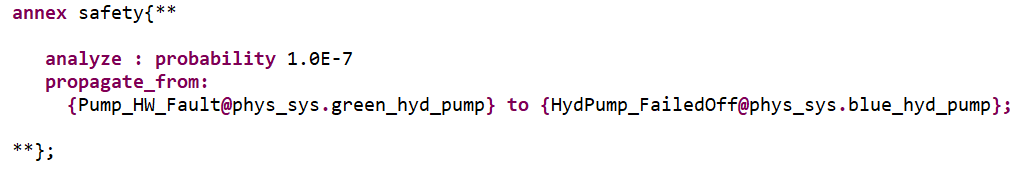
\includegraphics[width=1.0\textwidth]{images/hw_prop_stmt.png}
	\end{center}
	\vspace{-0.3in}
	%\caption{Hardware Fault Propagation Statement}
	\label{fig:hwFaultProp}
	%\vspace{-0.2in}
	\vspace{-0.1in}
\end{figure}

The fault dependencies are specified in the system implementation where the system configuration that causes the dependencies becomes clear (e.g., binding between SW and HW components, co-location of HW components). 
%This is because fault propagations are typically tied to the way components are connected or bound together; this information may not be available when faults are being specified for individual components. Having fault propagations specified outside of a component’s fault statements also makes it easier to reuse the component in different systems. 


\begin{comment}
\subsection{Fault Hypothesis}

An annotation in the AADL model determines the fault hypothesis. This may specify either a maximum number of faults that can be active at any point in execution (see Figure~\ref{fig:hwFaultProp}) or that only faults whose probability of simultaneous occurrence is above some probability threshold should be considered. Tying back to traditional safety analysis, the former is analogous to restricting the cutsets to a specified maximum number of terms, and the latter is analogous to restricting the cutsets to only those whose probability is above some set value.

In the former case, we assert that the sum of the true {\em fault\_\_trigger} variables is below some integer threshold.  In the latter, we determine all combinations of faults whose probabilities are above the specified probability threshold, and describe this as a proposition over {\em fault\_\_trigger} variables. 
%
With the introduction of dependent faults, active faults are divided into two categories: independently active (activated by its own triggering event) and dependently active (activated when the faults they depend on become active). The top level fault hypothesis applies to independently active faults. Faulty behaviors augment nominal behaviors whenever their corresponding faults are active (either independently active or dependently active).
\end{comment}










\section{Architecture and Implementation}
\label{sec:implementation}

The architecture of the Safety Annex is shown in Figure~\ref{fig:plugin-arch}.  It is written in Java as a plug-in for the OSATE AADL toolset, which is built on Eclipse.  It is not designed as a stand-alone extension of the language, but works with behavioral contracts specified in AGREE AADL annex and associated tools~\cite{NFM2012:CoGaMiWhLaLu}.  AGREE allows {\em assume-guarantee} behavioral contracts to be added to AADL components.  The language used for contract specification is based on the Lustre dataflow language~\cite{Halbwachs91:IEEE}. AGREE improves scalability of formal verification to large systems by decomposing the analysis of a complex system architecture into a collection of smaller verification tasks that correspond to the structure of the architecture.

\begin{figure}
	\begin{center}
		%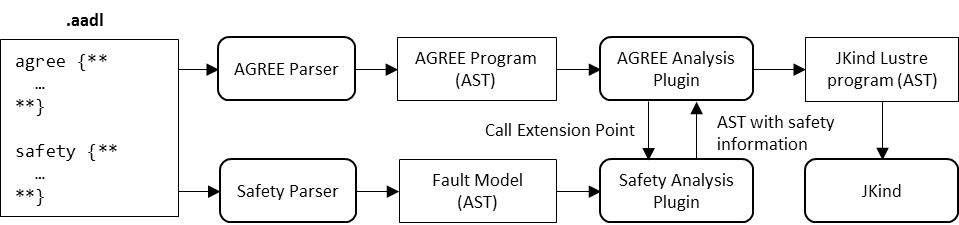
\includegraphics[trim=0 400 430 0,clip,width=0.85\textwidth]{images/arch.png}
		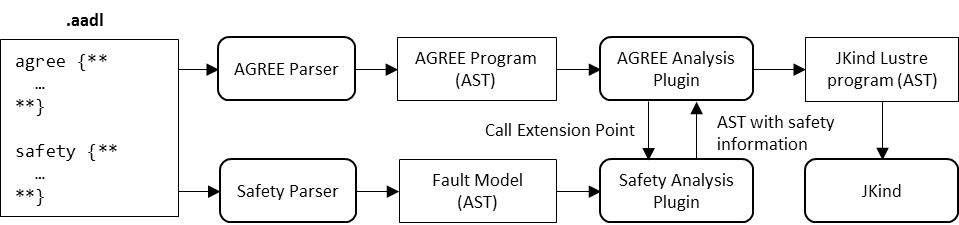
\includegraphics[width=.9\textwidth]{images/arch.png}
	\end{center}
	\vspace{-0.2in}
	\caption{Safety Annex Plug-in Architecture}
	\label{fig:plugin-arch}
\end{figure}

AGREE contracts are used to define the nominal behaviors of system components as {\em guarantees} that hold when {\em assumptions} about the values the component's environment are met.  The Safety Annex extends these contracts to allow faults to modify the behavior of component inputs and outputs.  To support these extensions, AGREE implements an Eclipse extension point interface that allows other plug-ins to modify the generated abstract syntax tree (AST) prior to its submission to the solver.  If the Safety Annex is enabled, these faults are added to the AGREE contract and, when triggered, override the nominal guarantees provided by the component.  

An example of a portion of an initial AGREE node and its extended contract is shown in Figure~\ref{fig:lustre}.  %The \texttt{\_\_fault} variables and declarations are added to allow the contract to override the nominal behavioral constraints (provided by guarantees) on outputs.  In the Lustre language, \texttt{assertion}s are constraints that are assumed to hold in the transition system. 
In the left column of the figure, the nominal Lustre pump definition is shown with an AGREE contract on the output. In the right column, the additional local variables for the fault are seen in boxes 1 and 2, the assertion binding the fault value to the nominal value is seen in boxes 3 and 4, and the fault node definition is given in box 5. 

%A  benefit of utilizing the AGREE behavioral annex is the ability to perform both monolithic and compositional analysis on the nominal model. AGREE allows {\em assume-guarantee} behavioral contracts to be added to AADL components.  The language used for contract specification is based on the Lustre dataflow language~\cite{Halbwachs91:IEEE} and the nominal model (AADL model annotated with AGREE contracts) is translated into Lustre before being sent to the JKind model checker for verification\cite{2017arXiv171201222G}. 

%When a user selects to run the fault analysis during verification, the AGREE contracts are automatically extended in Lustre in order to allow faults to modify the behavior of component outputs. These injections into the Lustre model are shown in Figure~\ref{fig:lustre}. 

\begin{figure}[h!]
	\hspace*{-2cm}
	\vspace{-0.3in} 
	\begin{center}
		%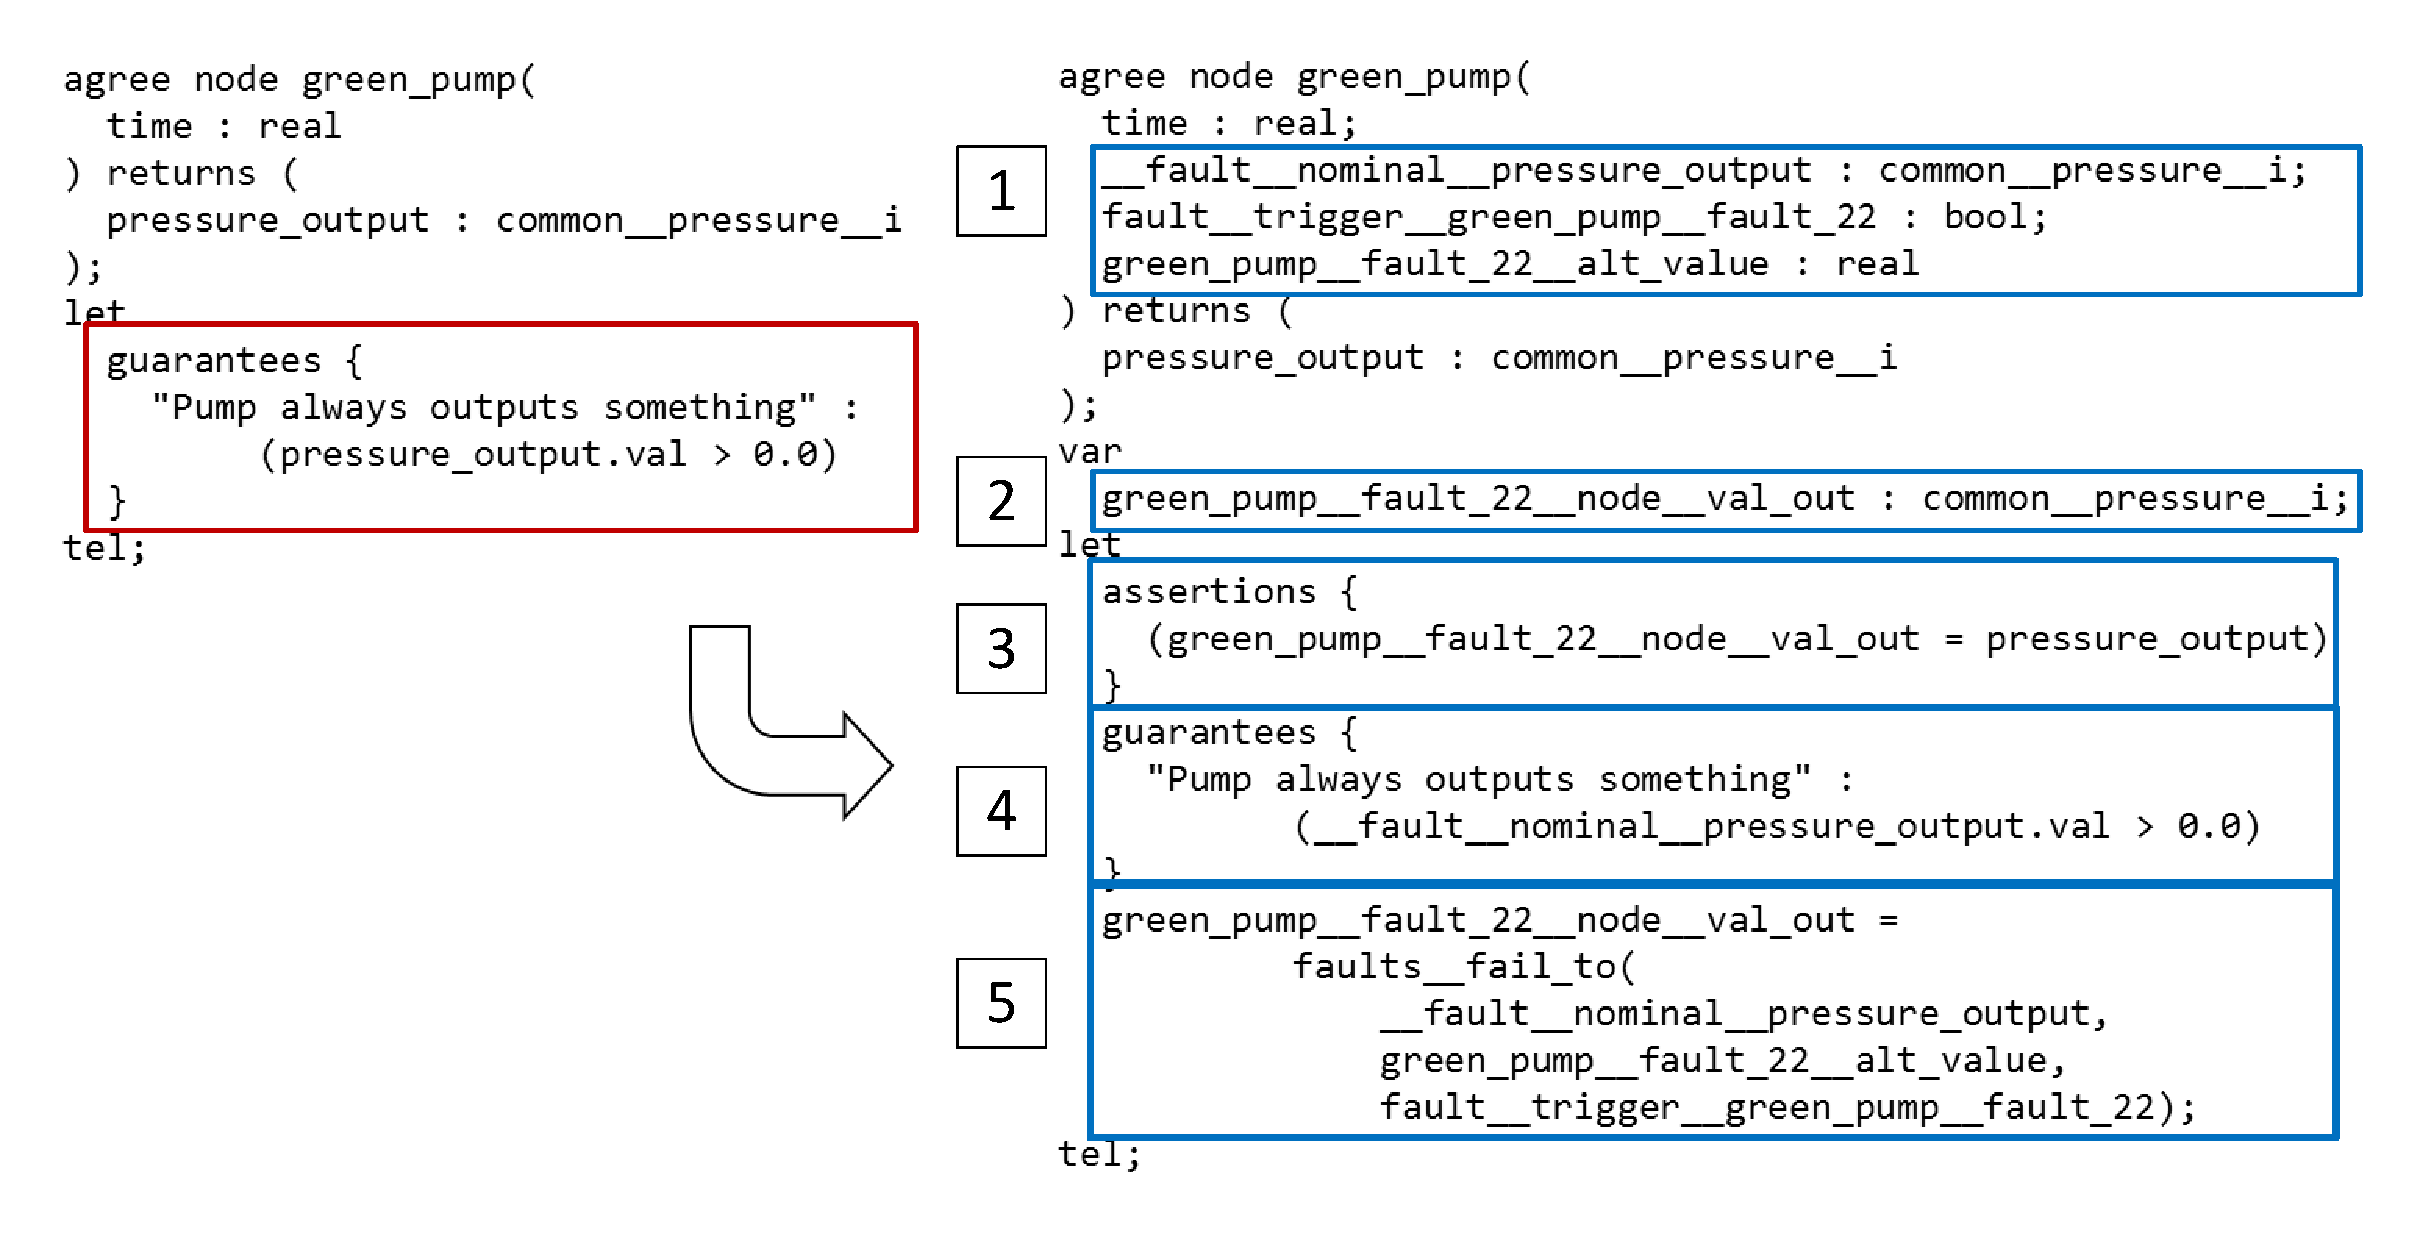
\includegraphics[trim=0 690 -10 70,clip,width=1.5\dimexpr\textwidth-2cm\relax]{images/lustre.pdf}
		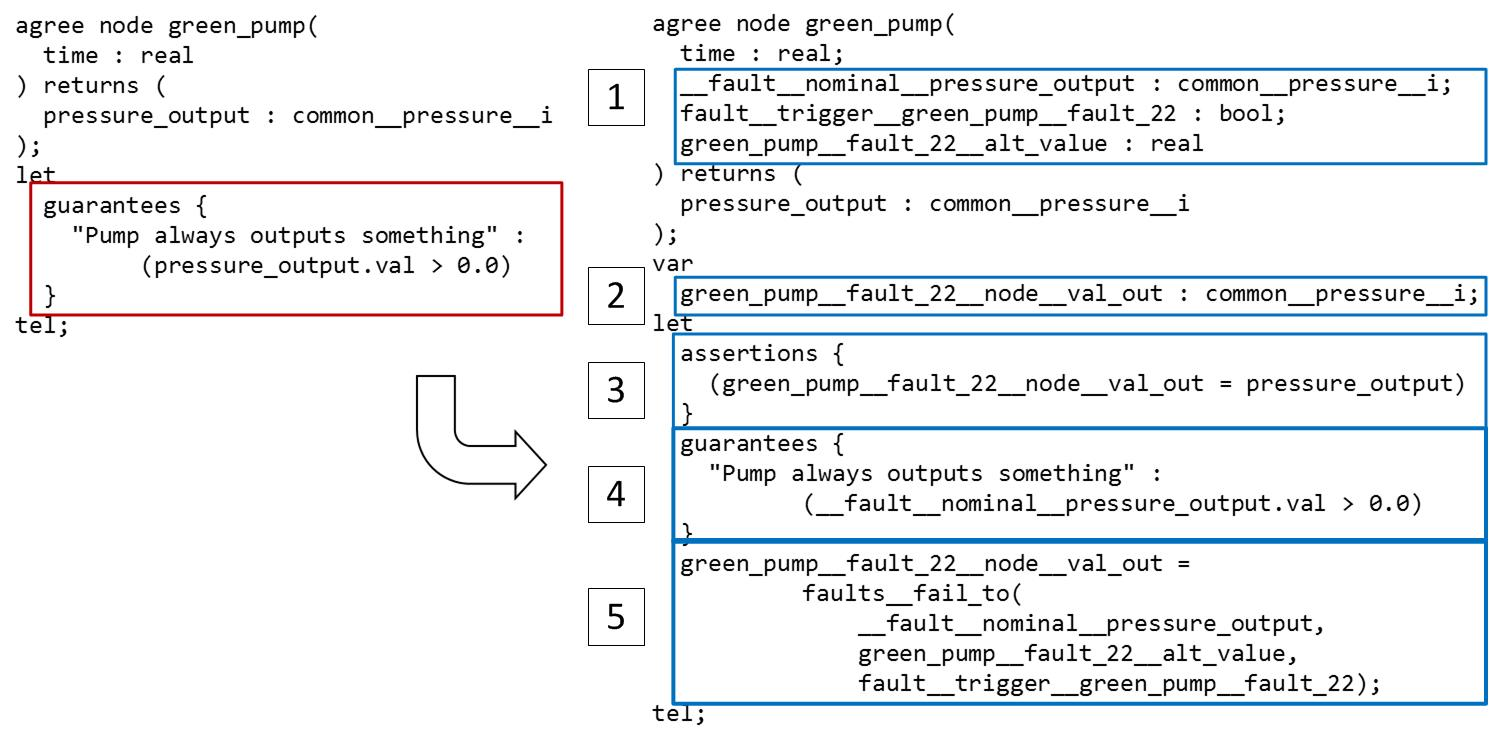
\includegraphics[scale=0.3]{images/lustre.jpg}
		\caption{Nominal AGREE node and its extension with faults}
		\label{fig:lustre}
	\end{center}
	\vspace{-0.3in}
\end{figure}

\begin{comment}
\begin{figure}
	\vspace{-0.1in}
	%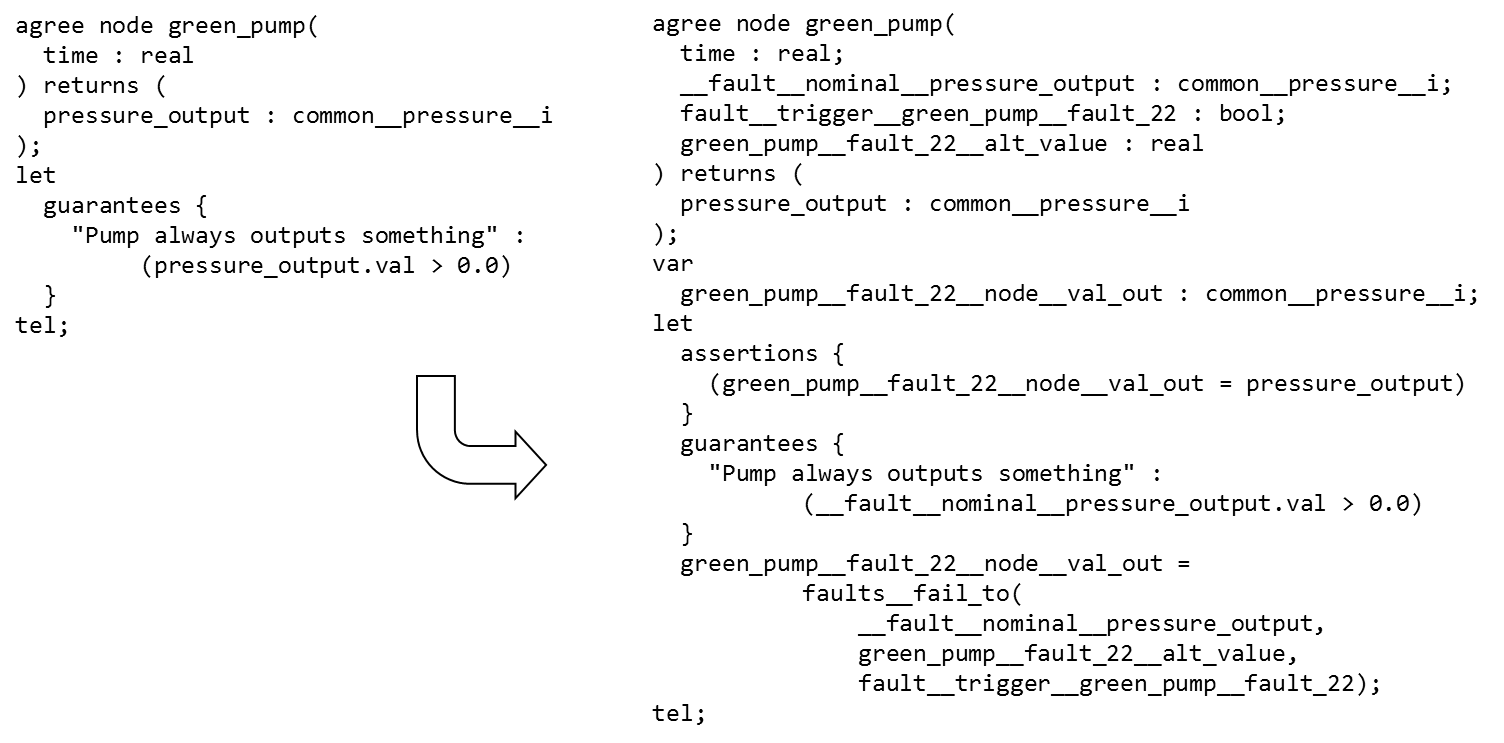
\includegraphics[trim=30 150 120 10,clip,width=\textwidth]{images/sample_code.png}
	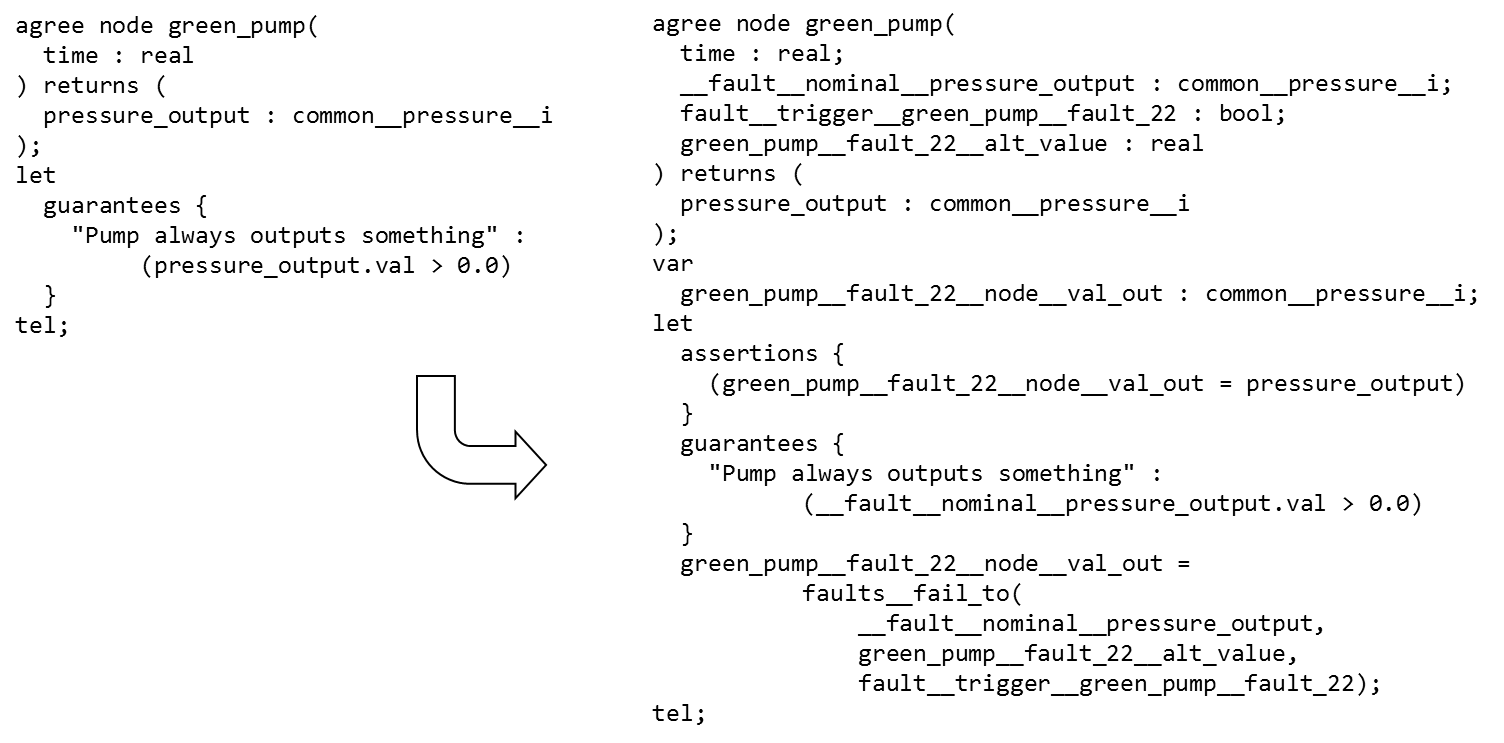
\includegraphics[width=\textwidth]{images/sample_code.png}
	\vspace{-0.3in}
	\caption{Nominal AGREE node and its extension with faults}
	\label{fig:comp}
\end{figure}
\end{comment}
%An annotation in the AADL model determines the fault hypothesis.  This may specify either a maximum number of faults that can be active at any point in execution (typically one or two), or that only faults whose probability of simultaneous occurrence is above some probability threshold should be considered. In the former case, we assert that the sum of the true {\em fault\_\_trigger} variables is below some integer threshold.  In the latter, we determine all combinations of faults whose probabilities are above the specified probability threshold, and describe this as a proposition over {\em fault\_\_trigger} variables.
%
%With the introduction of dependent faults, active faults are divided into two categories: independently active (activated by its own triggering event) and dependently active (activated when the faults they depend on become active). The top level fault hypothesis applies to independently active faults. Faulty behaviors augment nominal behaviors whenever their corresponding faults are active (either independently active or dependently active).

Once augmented with fault information, the AGREE model follows the standard translation path to the model checker JKind~\cite{2017arXiv171201222G}, an infinite-state model checker for safety properties.  The augmentation includes traceability information so that when counterexamples are displayed to users, the active faults for each component are visualized.


%For fault analysis, we separate the possible analyses available to users into two distinct actions and describe them here.


\section{Fault Model Analysis in the Shared Model Process}
\label{sec:fault_analysis_2}

To demonstrate the shared model process, we outline a subsystem of the WBS and describe the interaction between system development process and the system safety process using a shared model.   

\section{Related Work}
\label{sec:related_work}

%Address NFM review comments
In recent years, there has been an increase in the interest of Model Based Safety Analysis (MBSA)~\cite{Bozzano:2010:DSA:1951720}. 

Formal model based systems engineering (MBSE) methods and tools now permit system level requirements to be specified and analyzed early in the development process~\cite{QFCS15:backes,CIMATTI2015333, NFM2012:CoGaMiWhLaLu, hilt2013:MuWhRaHe, Pajic2012}. Design models from which aircraft systems are developed can be integrated into the safety analysis process to help guarantee accurate and consistent results. This integration is especially important as the amount of safety critical hardware and software has dramatically increased in safety critical domains such as aerospace, automotive, and medical fields~\cite{Stewart17:IMBSA}.

There are tools that currently support reasoning about faults in architecture description languages such as SysML and AADL. These tools include the AADL Error Model Annex, Version 2 (EMV2)~\cite{EMV2} and HiP-HOPS for EAST-ADL~\cite{CHEN201391}. These approaches primarily utilize \textit{qualitative} reasoning. Faults are enumerated and the propagations through system components are explicitly described. Given many possible faults, these propagation relationships increase in complexity and understandability. Interactions are easily overlooked by analysts and thus not explicitly described. This is also the case with tools like SAML that incorporate both \textit{qualitative} and \textit{quantitative} reasoning~\cite{Gudemann:2010:FQQ:1909626.1909813}. 

In earlier work, an approach to MBSA was demonstrated using the Simulink notation~\cite{Joshi05:SafeComp,Joshi05:Dasc,NasaRep:MBSA-Aug05, MathWorks} . In this approach, a behavioral model of system dynamics was used to reason about the effects of faults in the system. We believe this approach allows an implicit and natural notion of fault propagation through the system. Since Simulink is not an architecture description language, notions such as hardware devices and non-functional aspects cannot be captured in system models. Using this idea of \textit{quantitative} reasoning and implicit fault propagation, we wish to apply this to a more rich architecture language. 


Formal verification tools based on model checking have been used to automate the generation of safety artifacts and used in safety critical system certification~\cite{Bozzano:2011:SDP:1992983.1992988, symbAltaRica,10.1007/978-3-540-75596-8-13, DBLP:conf/tacas/BittnerBCCGGMMZ16, Bozzano:2010:DSA:1951720} . This approach has limitations in terms of scalability and readability of the fault trees generated. Work has been done to mitigate these limitations by the scalable generation of readable fault trees~\cite{10.1007/978-3-319-11936-6-7}. 

%Moved the following to case study
%The Wheel Brake System (WBS) described in ARP4761~\cite{SAE:ARP4761} has been used in the past as a case study for safety analysis, formal verification, and contract based design~\cite{DBLP:conf/cav/BozzanoCPJKPRT15, 10.1007/978-3-319-11936-6-7, CAV2015:BoCiGrMa, Stewart17:IMBSA, propBasedProofSys, Joshi05:SafeComp, NasaRep:MBSA-Aug05} The preliminary work for the safety annex used a simplified model of the WBS~\cite{Stewart17:IMBSA}. In order to show scalability and compare results with other studies, an AADL version of the WBS was designed based off of arch4wbs NuSMV model described in previous work~\cite{DBLP:conf/cav/BozzanoCPJKPRT15}. This model was chosen due to the number of subcomponents in the system and the complexity of behavior captured in the NuSMV model. 



\section{Conclusion}

We have developed an extension to the AADL language with tool support for formal analysis of system safety properties in the presence of faults. Faulty behavior is specified as an extension of the nominal model, allowing safety analysis and system implementation to be driven from a single common model. This new Safety Annex leverages the AADL structural model and nominal behavioral specification (using the AGREE annex) to propagate faulty component behaviors without the need to add separate propagation specifications to the model.   Next steps will include extensions to automate injection of Byzantine faults as well as automatic generation of fault trees.  For more details on the tool, models, and approach, see the technical report~\cite{SATechReport}.

\vspace{2 mm}
\noindent {\bf Acknowledgments.} This research was funded by NASA contract NNL16AB07T and the University of Minnesota College of Science and Engineering Graduate Fellowship.




\vspace{-0.40cm}
\bibliographystyle{abbrv}
\bibliography{biblio}
%\vspace{-7.25cm}
% This ~ seems to fix an odd bibliography alignment issue
~

%\ifdefined\TECHREPORT
%\appendix
%
%\section{Appendix: Proof of Equivalence}
%\input{appendix}
%\fi

%\section{Appendix: GPCA CENTA Model}
%\label{appendix:gpcacenta}
%\begin{figure}[!ht]
%\begin{center}
%\includegraphics[scale=0.6]{images/sampled_pca.PNG} %[trim = 0 2 0 0, clip=true]{Comp}
%\caption{GPCA AGREE Properties modeled as a Timed Automata} \label{fig:samplepca}
%\end{center}
%\end{figure}

%\balancecolumns

\end{document} 